\documentclass[hyperref, a4paper]{article}

\usepackage{geometry}
\usepackage{titling}
\usepackage{titlesec}
\usepackage{paralist}
\usepackage{footnote}
\usepackage{enumerate}
\usepackage{amsmath, amssymb, amsthm}
\usepackage{mathtools}
\usepackage{bbm}
\usepackage{cite}
\usepackage{graphicx}
\usepackage{subcaption}
\usepackage{physics}
\usepackage{siunitx}
\usepackage[version=4]{mhchem}
\usepackage{tikz}
\usepackage{xcolor}
\usepackage{listings}
\usepackage{autobreak}
\usepackage[ruled, vlined, linesnumbered, noend]{algorithm2e}
\usepackage[colorlinks]{hyperref} % , linkcolor=black, anchorcolor=black, citecolor=black, urlcolor=black
\usepackage{prettyref}

% Page style
\geometry{left=3.18cm,right=3.18cm,top=2.54cm,bottom=2.54cm}
\titlespacing{\paragraph}{0pt}{1pt}{10pt}[20pt]
\setlength{\droptitle}{-5em}
\preauthor{\vspace{-10pt}\begin{center}}
\postauthor{\par\end{center}}

% Math operators
\DeclareMathOperator{\timeorder}{T}
\DeclareMathOperator{\diag}{diag}
\DeclareMathOperator{\legpoly}{P}
\DeclareMathOperator{\primevalue}{P}
\DeclareMathOperator{\sgn}{sgn}
\newcommand*{\ii}{\mathrm{i}}
\newcommand*{\ee}{\mathrm{e}}
\newcommand*{\const}{\mathrm{const}}
\newcommand*{\suchthat}{\quad \text{s.t.} \quad}
\newcommand*{\argmin}{\arg\min}
\newcommand*{\argmax}{\arg\max}
\newcommand*{\normalorder}[1]{: #1 :}
\newcommand*{\pair}[1]{\langle #1 \rangle}
\newcommand*{\fd}[1]{\mathcal{D} #1}
\DeclareMathOperator{\bigO}{\mathcal{O}}

% TikZ setting
\usetikzlibrary{arrows,shapes,positioning}
\usetikzlibrary{arrows.meta}
\usetikzlibrary{decorations.markings}
\tikzstyle arrowstyle=[scale=1]
\tikzstyle directed=[postaction={decorate,decoration={markings,
    mark=at position .5 with {\arrow[arrowstyle]{stealth}}}}]
\tikzstyle ray=[directed, thick]
\tikzstyle dot=[anchor=base,fill,circle,inner sep=1pt]

% Algorithm setting
% Python-style code
\SetKwIF{If}{ElseIf}{Else}{if}{:}{elif:}{else:}{}
\SetKwFor{For}{for}{:}{}
\SetKwFor{While}{while}{:}{}
\SetArgSty{textnormal}

\newcommand*{\concept}[1]{{\textbf{#1}}}

\lstset{basicstyle=\ttfamily,
  showstringspaces=false,
  commentstyle=\color{gray},
  keywordstyle=\color{blue}
}

\newcommand*{\Ztwo}{$\mathbb{Z}_2$ }
\newcommand*{\tfim}{transverse field Ising model }
\newcommand*{\cim}{classical Ising model }

\title{\Ztwo Gauge Field Coupled to a Fermion System}
\author{Jinyuan Wu}

\begin{document}

\maketitle

In the whole article we use $\sigma$ and $s$ as shorthands of $\sigma^z$ and $s^z$, unless confusion may be caused by the notation.

\section{The model Hamiltonian}

The model investigated in this article is shown in \cite{moon2019deconfined}.
The model Hamiltonian is 
\begin{equation}
    H = H_Z \underbrace{- J \sum_{\pair{\vb*{i}, \vb*{j}}} \sigma_{\vb*{i} \vb*{j}} s_{\vb*{i}} s_{\vb*{j}} + \sum_i h^x_i s^x_i}_{H_\text{Ising}} - t \sum_{\pair{\vb*{i}, \vb*{j}}} \sigma_{\vb*{i} \vb*{j}} c^\dagger_{\vb*{i}} c_{\vb*{j}},
    \label{eq:proposed-model}
\end{equation}
where
\begin{equation}
    H_Z = - g \sum_{\vb*{l} \in \Box_{\vb*{i}^*}} \sigma_{\vb*{i} \vb*{j}}^z - h \sum_{\pair{\vb*{i}, \vb*{j}}} \sigma^x_{\vb*{i} \vb*{j}}, 
\end{equation}
where $\vb*{i}^*$ is a site in the dual lattice (i.e. a site placed at the center of a plaquette), 
$\Box_{\vb*{i}^*}$ is the plaquette whose center is $\vb*{i}^*$, and $\vb*{l}$ denotes a certain bond of a plaquette.
Such kind of model Hamiltonian usually emerges from orthogonal metals \cite{moon2019deconfined, orthogonal_metal}.

In this section, we introduce every part of \eqref{eq:proposed-model}.

\subsection{\Ztwo gauge field and its dual theories}

\subsubsection{The plaquette term}

\begin{figure}
    \centering
    

\tikzset{every picture/.style={line width=0.75pt}} %set default line width to 0.75pt        

\begin{tikzpicture}[x=0.75pt,y=0.75pt,yscale=-1,xscale=1]
%uncomment if require: \path (0,300); %set diagram left start at 0, and has height of 300

%Shape: Square [id:dp4522225054629818] 
\draw  [fill={rgb, 255:red, 255; green, 0; blue, 0 }  ,fill opacity=0.25 ] (268,149) -- (318,149) -- (318,199) -- (268,199) -- cycle ;
%Shape: Square [id:dp4594732045911669] 
\draw  [fill={rgb, 255:red, 0; green, 0; blue, 255 }  ,fill opacity=0.25 ] (168,99) -- (218,99) -- (218,149) -- (168,149) -- cycle ;
%Straight Lines [id:da7859210255370197] 
\draw    (168,99) -- (218,99) ;
%Straight Lines [id:da12886428106250913] 
\draw    (168,149) -- (218,149) ;
%Straight Lines [id:da5836673303401485] 
\draw    (168,149) -- (168,99) ;
%Straight Lines [id:da6832798720040101] 
\draw    (218,149) -- (218,99) ;
%Shape: Square [id:dp4552383640295201] 
\draw   (168,99) -- (218,99) -- (218,149) -- (168,149) -- cycle ;
%Shape: Square [id:dp4299395977342566] 
\draw   (218,99) -- (268,99) -- (268,149) -- (218,149) -- cycle ;
%Shape: Square [id:dp7609749847711793] 
\draw   (218,149) -- (268,149) -- (268,199) -- (218,199) -- cycle ;
%Shape: Square [id:dp7189104654045673] 
\draw   (268,149) -- (318,149) -- (318,199) -- (268,199) -- cycle ;
%Shape: Square [id:dp3279496623171845] 
\draw   (168,149) -- (218,149) -- (218,199) -- (168,199) -- cycle ;
%Shape: Square [id:dp09533953088675018] 
\draw   (268,99) -- (318,99) -- (318,149) -- (268,149) -- cycle ;
%Shape: Square [id:dp6743217671924511] 
\draw  [color={rgb, 255:red, 144; green, 19; blue, 254 }  ,draw opacity=1 ][line width=2.25]  (168,99) -- (218,99) -- (218,149) -- (168,149) -- cycle ;
%Straight Lines [id:da23601359728908688] 
\draw [color={rgb, 255:red, 0; green, 0; blue, 0 }  ,draw opacity=1 ]   (189.64,112.54) -- (195.88,87.4) ;
\draw [shift={(196.36,85.46)}, rotate = 463.92] [fill={rgb, 255:red, 0; green, 0; blue, 0 }  ,fill opacity=1 ][line width=0.08]  [draw opacity=0] (12,-3) -- (0,0) -- (12,3) -- cycle    ;
%Straight Lines [id:da8963244134502486] 
\draw [color={rgb, 255:red, 0; green, 0; blue, 0 }  ,draw opacity=1 ]   (164.64,110.46) -- (170.88,135.6) ;
\draw [shift={(171.36,137.54)}, rotate = 256.08] [fill={rgb, 255:red, 0; green, 0; blue, 0 }  ,fill opacity=1 ][line width=0.08]  [draw opacity=0] (12,-3) -- (0,0) -- (12,3) -- cycle    ;
%Straight Lines [id:da6667388980914568] 
\draw [color={rgb, 255:red, 0; green, 0; blue, 0 }  ,draw opacity=1 ]   (189.64,135.46) -- (195.88,160.6) ;
\draw [shift={(196.36,162.54)}, rotate = 256.08] [fill={rgb, 255:red, 0; green, 0; blue, 0 }  ,fill opacity=1 ][line width=0.08]  [draw opacity=0] (12,-3) -- (0,0) -- (12,3) -- cycle    ;
%Straight Lines [id:da015522846808282864] 
\draw [color={rgb, 255:red, 0; green, 0; blue, 0 }  ,draw opacity=1 ]   (214.64,110.46) -- (220.88,135.6) ;
\draw [shift={(221.36,137.54)}, rotate = 256.08] [fill={rgb, 255:red, 0; green, 0; blue, 0 }  ,fill opacity=1 ][line width=0.08]  [draw opacity=0] (12,-3) -- (0,0) -- (12,3) -- cycle    ;
%Shape: Square [id:dp05679192513289277] 
\draw  [color={rgb, 255:red, 208; green, 2; blue, 27 }  ,draw opacity=1 ][line width=2.25]  (268,149) -- (318,149) -- (318,199) -- (268,199) -- cycle ;
%Straight Lines [id:da21391036278901998] 
\draw [color={rgb, 255:red, 0; green, 0; blue, 0 }  ,draw opacity=1 ]   (289.04,162.54) -- (295.28,137.4) ;
\draw [shift={(295.76,135.46)}, rotate = 463.92] [fill={rgb, 255:red, 0; green, 0; blue, 0 }  ,fill opacity=1 ][line width=0.08]  [draw opacity=0] (12,-3) -- (0,0) -- (12,3) -- cycle    ;
%Straight Lines [id:da9816247930379984] 
\draw [color={rgb, 255:red, 0; green, 0; blue, 0 }  ,draw opacity=1 ]   (289.04,185.46) -- (295.28,210.6) ;
\draw [shift={(295.76,212.54)}, rotate = 256.08] [fill={rgb, 255:red, 0; green, 0; blue, 0 }  ,fill opacity=1 ][line width=0.08]  [draw opacity=0] (12,-3) -- (0,0) -- (12,3) -- cycle    ;
%Straight Lines [id:da31464719110814876] 
\draw [color={rgb, 255:red, 0; green, 0; blue, 0 }  ,draw opacity=1 ]   (314.04,160.46) -- (320.28,185.6) ;
\draw [shift={(320.76,187.54)}, rotate = 256.08] [fill={rgb, 255:red, 0; green, 0; blue, 0 }  ,fill opacity=1 ][line width=0.08]  [draw opacity=0] (12,-3) -- (0,0) -- (12,3) -- cycle    ;
%Straight Lines [id:da8559300619509063] 
\draw [color={rgb, 255:red, 0; green, 0; blue, 0 }  ,draw opacity=1 ]   (265.84,187.74) -- (272.08,162.6) ;
\draw [shift={(272.56,160.66)}, rotate = 463.92] [fill={rgb, 255:red, 0; green, 0; blue, 0 }  ,fill opacity=1 ][line width=0.08]  [draw opacity=0] (12,-3) -- (0,0) -- (12,3) -- cycle    ;
%Straight Lines [id:da015254394235462598] 
\draw    (135.33,228.33) -- (183.33,228.33) ;
\draw [shift={(185.33,228.33)}, rotate = 180] [fill={rgb, 255:red, 0; green, 0; blue, 0 }  ][line width=0.08]  [draw opacity=0] (12,-3) -- (0,0) -- (12,3) -- cycle    ;
%Straight Lines [id:da5713451115525661] 
\draw    (135.33,228.33) -- (135.33,180.33) ;
\draw [shift={(135.33,178.33)}, rotate = 450] [fill={rgb, 255:red, 0; green, 0; blue, 0 }  ][line width=0.08]  [draw opacity=0] (12,-3) -- (0,0) -- (12,3) -- cycle    ;

% Text Node
\draw (193,124) node    {$-1$};
% Text Node
\draw (293,174) node    {$1$};
% Text Node
\draw (293,124) node    {$\boldsymbol{i}^{*}$};
% Text Node
\draw (266,145.6) node [anchor=south east] [inner sep=0.75pt]    {$\boldsymbol{i}$};
% Text Node
\draw (187.33,228.33) node [anchor=west] [inner sep=0.75pt]    {$x$};
% Text Node
\draw (135.45,174.94) node [anchor=south] [inner sep=0.75pt]  [rotate=-2]  {$y$};


\end{tikzpicture}

    \caption{A \Ztwo gauge field configuration. The blue plaquette's $F_{\vb*{i}^*}$ is $(-1) \times 1 \times (-1) \times (-1) = -1$, %
    while the red plaquette's $F_{\vb*{i}^*}$ is $1 \times 1 \times (-1) \times (-1) = 1$. %
    Note that we assign the same index to a plaquette's center (labeled as $\vb*{i}^*$ at the right top of the diagram) %
    and the plaquette's left bottom site $\vb*{i}$. %
    The terms ``up'' and ``down'' are defined in the Cartesian coordinates given in the diagram.}
    \label{fig:z2-gauge-field}
\end{figure}

The plaquette term in the Hamiltonian of the \Ztwo gauge field is be a function of
\begin{equation}
    F_{i^*} = \prod_{l \in \Box_{i^*}} \sigma_l,
\end{equation}
which is invariant under a \Ztwo gauge transformation
\begin{equation}
    Q_{\vb*{i}} = \prod_{\vb*{l} \in +_{\vb*{i}}} \sigma^x_{\vb*{l}}.
\end{equation}
A convenient convention is to let a plaquette share the same index with the site in its left bottom corner. 
An example of a \Ztwo gauge field configuration can be found in \prettyref{fig:z2-gauge-field}.

\subsubsection{The transverse field}

We name the \Ztwo gauge theory with plaquette terms only as the \concept{Wegner model}, i.e.
\begin{equation}
    H_\text{W} = - g \sum_{\vb*{i}} F_{{\vb*{i}}^*}.
\end{equation}
There is no quantum fluctuation in $H_\text{W}$. 
The existence of interaction between the \Ztwo field and the Ising field and the fermions introduces effective interaction channels between \Ztwo excitations, but all effective interaction between \Ztwo excitations are in terms of $\sigma^z_{\vb*{i} \vb*{j}}$, which commutes with $H_Z$ and therefore do not bring in quantum fluctuation.

An idiomatic way to add quantum fluctuation is to add a transverse field.
In this project we consider a transverse field Hamiltonian in the form of 
\begin{equation}
    H_h = - h \sum_{\pair{\vb*{i}, \vb*{j}}} \sigma_{\vb*{i} \vb*{j}}^x ,
    \label{eq:transverse-field}
\end{equation}
where the parameter $h$ measures the quantum fluctuation.
\eqref{eq:transverse-field} obviously commutes with $\vb*{Q}_{\vb*{i}}$ for every $\vb*{i}$, so it can be a term in a \Ztwo gauge invariant Hamiltonian. 
In the language of string-net condensation, $H_h$ is a string tension term.
So when we say ``\Ztwo gauge theory'', usually we are referring to 
\begin{equation}
    H = - J \sum_{\vb*{i}} \prod_{\vb*{l} \in \Box_{\vb*{i}^*}} \sigma_{\vb*{l}} - h \sum_{\pair{\vb*{i}, \vb*{j}}} \sigma_{\vb*{i} \vb*{j}}^x.
    \label{eq:standard-z2-theory}
\end{equation}

\subsubsection{Equivalence between a \Ztwo gauge theory when $h = 0$ and a bundle of Ising chains}

Now we consider a \Ztwo field theory with the plaquette term only, or in other words, we investigate the Wegner model.
With the gauge choice
\begin{equation}
    \sigma_{\vb*{i}, \vb*{i}+\vu*{x}} = 1,
    \label{eq:gauge-choice-x}
\end{equation}
we have
\begin{equation}
    F_{i^*} = \sigma_{i, i+\hat{y}} \sigma_{i+\hat{x}, i + \hat{x} + \hat{y}},
\end{equation}
which, by renaming $\sigma_{i, i+\hat{y}}$ into $S_i$, reads 
\begin{equation}
    F_{i^*} = S_i S_{i+\hat{x}}.
\end{equation}
The hopping constant $\sigma_{\vb*{i} \vb*{j}}$, respectively, is
\begin{equation}
    \sigma_{\vb*{i} \vb*{j}} = \left\{
    \begin{aligned}
        1, &\quad j = i + \hat{x}, \\
        S_i, &\quad j = i + \hat{y},
    \end{aligned}
\right., \quad \sigma_{\vb*{j} \vb*{i}} = \sigma_{\vb*{i} \vb*{j}}.
\end{equation}

This, actually, means that the \Ztwo gauge field may also be transformed into a dual transverse field Ising field.
For example consider Wegner model.
With the definition of $S_i$s it is rephrased into
\begin{equation}
    H_\text{W} = -g \sum_i S_i S_{i+\hat{x}},
\end{equation}
so the model is actually a bundle of 1D Ising spin chain.

\begin{figure}
    \centering
    

\tikzset{every picture/.style={line width=0.75pt}} %set default line width to 0.75pt        

\begin{tikzpicture}[x=0.75pt,y=0.75pt,yscale=-1,xscale=1]
%uncomment if require: \path (0,300); %set diagram left start at 0, and has height of 300

%Shape: Square [id:dp09479692823165653] 
\draw   (153.33,57) -- (203.33,57) -- (203.33,107) -- (153.33,107) -- cycle ;
%Shape: Square [id:dp5110721328962706] 
\draw   (253.33,107) -- (303.33,107) -- (303.33,157) -- (253.33,157) -- cycle ;
%Shape: Square [id:dp596441711528124] 
\draw   (203.33,107) -- (253.33,107) -- (253.33,157) -- (203.33,157) -- cycle ;
%Shape: Square [id:dp6284614343612833] 
\draw   (153.33,107) -- (203.33,107) -- (203.33,157) -- (153.33,157) -- cycle ;
%Shape: Square [id:dp6055477074062259] 
\draw   (253.33,57) -- (303.33,57) -- (303.33,107) -- (253.33,107) -- cycle ;
%Shape: Square [id:dp9978271567947337] 
\draw   (203.33,57) -- (253.33,57) -- (253.33,107) -- (203.33,107) -- cycle ;
%Straight Lines [id:da7733656001603588] 
\draw    (153.33,57) -- (153.33,107) ;
%Straight Lines [id:da305284209513327] 
\draw    (203.33,57) -- (253.33,57) ;
%Straight Lines [id:da03895057037521843] 
\draw    (253.33,57) -- (303.33,57) ;
%Straight Lines [id:da746243903528131] 
\draw    (153.33,107) -- (203.33,107) ;
%Straight Lines [id:da9628631915863632] 
\draw    (203.33,107) -- (253.33,107) ;
%Straight Lines [id:da8327728881661582] 
\draw    (253.33,107) -- (303.33,107) ;
%Straight Lines [id:da6159316366604941] 
\draw    (153.33,157) -- (203.33,157) ;
%Straight Lines [id:da5535342779227095] 
\draw    (203.33,157) -- (253.33,157) ;
%Straight Lines [id:da46622469228914865] 
\draw    (253.33,157) -- (303.33,157) ;
%Straight Lines [id:da07485445266898072] 
\draw    (153.33,107) -- (153.33,157) ;
%Straight Lines [id:da6485352210476978] 
\draw    (203.33,57) -- (203.33,107) ;
%Straight Lines [id:da45990260218715706] 
\draw    (203.33,107) -- (203.33,157) ;
%Straight Lines [id:da9933599692693724] 
\draw    (253.33,57) -- (253.33,107) ;
%Straight Lines [id:da048810688374390176] 
\draw    (253.33,107) -- (253.33,157) ;
%Straight Lines [id:da6712273461119682] 
\draw    (303.33,57) -- (303.33,107) ;
%Straight Lines [id:da46341727204361227] 
\draw    (303.33,107) -- (303.33,157) ;
%Straight Lines [id:da04201828049954481] 
\draw [color={rgb, 255:red, 0; green, 0; blue, 0 }  ,draw opacity=1 ]   (224.98,70.54) -- (231.21,45.4) ;
\draw [shift={(231.69,43.46)}, rotate = 463.92] [fill={rgb, 255:red, 0; green, 0; blue, 0 }  ,fill opacity=1 ][line width=0.08]  [draw opacity=0] (12,-3) -- (0,0) -- (12,3) -- cycle    ;
%Straight Lines [id:da48930485080929387] 
\draw [color={rgb, 255:red, 0; green, 0; blue, 0 }  ,draw opacity=1 ]   (174.98,70.54) -- (181.21,45.4) ;
\draw [shift={(181.69,43.46)}, rotate = 463.92] [fill={rgb, 255:red, 0; green, 0; blue, 0 }  ,fill opacity=1 ][line width=0.08]  [draw opacity=0] (12,-3) -- (0,0) -- (12,3) -- cycle    ;
%Straight Lines [id:da5751072992703958] 
\draw    (153.33,57) -- (203.33,57) ;
%Straight Lines [id:da45602531079114894] 
\draw [color={rgb, 255:red, 0; green, 0; blue, 0 }  ,draw opacity=1 ]   (274.98,70.54) -- (281.21,45.4) ;
\draw [shift={(281.69,43.46)}, rotate = 463.92] [fill={rgb, 255:red, 0; green, 0; blue, 0 }  ,fill opacity=1 ][line width=0.08]  [draw opacity=0] (12,-3) -- (0,0) -- (12,3) -- cycle    ;
%Straight Lines [id:da7435304597626089] 
\draw [color={rgb, 255:red, 0; green, 0; blue, 0 }  ,draw opacity=1 ]   (174.98,120.54) -- (181.21,95.4) ;
\draw [shift={(181.69,93.46)}, rotate = 463.92] [fill={rgb, 255:red, 0; green, 0; blue, 0 }  ,fill opacity=1 ][line width=0.08]  [draw opacity=0] (12,-3) -- (0,0) -- (12,3) -- cycle    ;
%Straight Lines [id:da7674561808153557] 
\draw [color={rgb, 255:red, 0; green, 0; blue, 0 }  ,draw opacity=1 ]   (224.98,120.54) -- (231.21,95.4) ;
\draw [shift={(231.69,93.46)}, rotate = 463.92] [fill={rgb, 255:red, 0; green, 0; blue, 0 }  ,fill opacity=1 ][line width=0.08]  [draw opacity=0] (12,-3) -- (0,0) -- (12,3) -- cycle    ;
%Straight Lines [id:da8426840224792957] 
\draw [color={rgb, 255:red, 0; green, 0; blue, 0 }  ,draw opacity=1 ]   (274.98,120.54) -- (281.21,95.4) ;
\draw [shift={(281.69,93.46)}, rotate = 463.92] [fill={rgb, 255:red, 0; green, 0; blue, 0 }  ,fill opacity=1 ][line width=0.08]  [draw opacity=0] (12,-3) -- (0,0) -- (12,3) -- cycle    ;
%Straight Lines [id:da4067239305634134] 
\draw [color={rgb, 255:red, 0; green, 0; blue, 0 }  ,draw opacity=1 ]   (174.98,170.54) -- (181.21,145.4) ;
\draw [shift={(181.69,143.46)}, rotate = 463.92] [fill={rgb, 255:red, 0; green, 0; blue, 0 }  ,fill opacity=1 ][line width=0.08]  [draw opacity=0] (12,-3) -- (0,0) -- (12,3) -- cycle    ;
%Straight Lines [id:da4465941343620421] 
\draw [color={rgb, 255:red, 0; green, 0; blue, 0 }  ,draw opacity=1 ]   (224.98,170.54) -- (231.21,145.4) ;
\draw [shift={(231.69,143.46)}, rotate = 463.92] [fill={rgb, 255:red, 0; green, 0; blue, 0 }  ,fill opacity=1 ][line width=0.08]  [draw opacity=0] (12,-3) -- (0,0) -- (12,3) -- cycle    ;
%Straight Lines [id:da19208047077894674] 
\draw [color={rgb, 255:red, 0; green, 0; blue, 0 }  ,draw opacity=1 ]   (274.98,170.54) -- (281.21,145.4) ;
\draw [shift={(281.69,143.46)}, rotate = 463.92] [fill={rgb, 255:red, 0; green, 0; blue, 0 }  ,fill opacity=1 ][line width=0.08]  [draw opacity=0] (12,-3) -- (0,0) -- (12,3) -- cycle    ;
%Shape: Square [id:dp5904563571752326] 
\draw  [draw opacity=0][fill={rgb, 255:red, 0; green, 0; blue, 255 }  ,fill opacity=0.25 ] (203.2,56.6) -- (253.2,56.6) -- (253.2,106.6) -- (203.2,106.6) -- cycle ;

%Shape: Square [id:dp6727604621907244] 
\draw  [draw opacity=0][fill={rgb, 255:red, 255; green, 0; blue, 0 }  ,fill opacity=0.25 ] (153.67,56.73) -- (203.67,56.73) -- (203.67,106.73) -- (153.67,106.73) -- cycle ;

%Straight Lines [id:da46103631391750355] 
\draw [color={rgb, 255:red, 0; green, 0; blue, 0 }  ,draw opacity=1 ]   (149.98,68.46) -- (156.21,93.6) ;
\draw [shift={(156.69,95.54)}, rotate = 256.08] [fill={rgb, 255:red, 0; green, 0; blue, 0 }  ,fill opacity=1 ][line width=0.08]  [draw opacity=0] (12,-3) -- (0,0) -- (12,3) -- cycle    ;
%Straight Lines [id:da04140473232568964] 
\draw [color={rgb, 255:red, 0; green, 0; blue, 0 }  ,draw opacity=1 ]   (199.98,68.46) -- (206.21,93.6) ;
\draw [shift={(206.69,95.54)}, rotate = 256.08] [fill={rgb, 255:red, 0; green, 0; blue, 0 }  ,fill opacity=1 ][line width=0.08]  [draw opacity=0] (12,-3) -- (0,0) -- (12,3) -- cycle    ;
%Straight Lines [id:da3032799741722214] 
\draw [color={rgb, 255:red, 0; green, 0; blue, 0 }  ,draw opacity=1 ]   (249.98,95.54) -- (256.21,70.4) ;
\draw [shift={(256.69,68.46)}, rotate = 463.92] [fill={rgb, 255:red, 0; green, 0; blue, 0 }  ,fill opacity=1 ][line width=0.08]  [draw opacity=0] (12,-3) -- (0,0) -- (12,3) -- cycle    ;
%Shape: Rectangle [id:dp11230349226059677] 
\draw  [draw opacity=0][fill={rgb, 255:red, 248; green, 231; blue, 28 }  ,fill opacity=0.33 ] (133.1,69.07) -- (323.3,69.07) -- (323.3,94.12) -- (133.1,94.12) -- cycle ;
%Straight Lines [id:da6808214285963194] 
\draw [color={rgb, 255:red, 0; green, 0; blue, 0 }  ,draw opacity=1 ]   (299.98,95.54) -- (306.21,70.4) ;
\draw [shift={(306.69,68.46)}, rotate = 463.92] [fill={rgb, 255:red, 0; green, 0; blue, 0 }  ,fill opacity=1 ][line width=0.08]  [draw opacity=0] (12,-3) -- (0,0) -- (12,3) -- cycle    ;
%Shape: Square [id:dp5830950799278609] 
\draw  [draw opacity=0][fill={rgb, 255:red, 255; green, 0; blue, 0 }  ,fill opacity=0.25 ] (253.67,57.13) -- (303.67,57.13) -- (303.67,107.13) -- (253.67,107.13) -- cycle ;

%Straight Lines [id:da8391598934215108] 
\draw    (110,191.67) -- (158,191.67) ;
\draw [shift={(160,191.67)}, rotate = 180] [fill={rgb, 255:red, 0; green, 0; blue, 0 }  ][line width=0.08]  [draw opacity=0] (12,-3) -- (0,0) -- (12,3) -- cycle    ;
%Straight Lines [id:da5618794888034828] 
\draw    (110,191.67) -- (110,143.67) ;
\draw [shift={(110,141.67)}, rotate = 450] [fill={rgb, 255:red, 0; green, 0; blue, 0 }  ][line width=0.08]  [draw opacity=0] (12,-3) -- (0,0) -- (12,3) -- cycle    ;

% Text Node
\draw (178.67,81.73) node    {$1$};
% Text Node
\draw (228.2,81.6) node    {$-1$};
% Text Node
\draw (278.67,82.13) node    {$1$};
% Text Node
\draw (162,191.67) node [anchor=west] [inner sep=0.75pt]    {$x$};
% Text Node
\draw (110.12,138.27) node [anchor=south] [inner sep=0.75pt]  [rotate=-2]  {$y$};


\end{tikzpicture}

    \caption{Converting a \Ztwo gauge field theory into a bundle of Ising chains. There is no interaction between parallel Ising chains.}
\end{figure}

\subsubsection{Mapping a \Ztwo gauge theory into a 2D \tfim}

\begin{equation}
    H = - h \sum_{\pair{\vb*{I}, \vb*{J}}} \tau^z_{\vb*{I}} \tau^z_{\vb*{J}} - J \sum_{\vb*{I}} \tau^x_{\vb*{I}}.
    \label{eq:z2-dual-theory}
\end{equation}

\eqref{eq:z2-dual-theory} is often called the \concept{dual \tfim} of \Ztwo gauge theory \eqref{eq:standard-z2-theory}.

\subsubsection{Absence of a finite temperature deconfined phase}\label{sec:absence-of-z2-deconfined-phase}

When $T=0$ and $h \ll g$, the \Ztwo gauge field exhibits a \emph{deconfined} phase, i.e. there are freely moving \Ztwo excitations such as \Ztwo fluxes.

When $h = 0$, the absence of quantum fluctuation here means the model is indeed totally classical, so there is no thermal phase transition, because a 1D Ising chain does not show thermal phase transition.
On the other hand, we know when $T=0$ the model exhibits deconfined \Ztwo charges, and when a transverse field is introduced a zero temperature quantum phase transition can be observed from the deconfined phase into the confined phase as the transverse field grows.
If for $T > 0$ there exists a deconfined phase, a simple analysis of the phase diagram tells us there must be a thermal phase transition when there is no transverse field.
The fact that Wegner model is dual to a bundle of 1D Ising chain and therefore lacks thermal phase transition implies that no deconfined phase exists with finite non zero temperature.

\begin{figure}
    \centering
    

\tikzset{every picture/.style={line width=0.75pt}} %set default line width to 0.75pt        

\begin{tikzpicture}[x=0.75pt,y=0.75pt,yscale=-1,xscale=1]
%uncomment if require: \path (0,300); %set diagram left start at 0, and has height of 300

%Straight Lines [id:da6058174087985544] 
\draw    (155.33,248.33) -- (359.89,248.33) ;
\draw [shift={(361.89,248.33)}, rotate = 180] [fill={rgb, 255:red, 0; green, 0; blue, 0 }  ][line width=0.08]  [draw opacity=0] (12,-3) -- (0,0) -- (12,3) -- cycle    ;
%Straight Lines [id:da3876935202277678] 
\draw    (155.33,248.33) -- (155.33,79.85) ;
\draw [shift={(155.33,77.85)}, rotate = 450] [fill={rgb, 255:red, 0; green, 0; blue, 0 }  ][line width=0.08]  [draw opacity=0] (12,-3) -- (0,0) -- (12,3) -- cycle    ;
%Straight Lines [id:da6788890136308154] 
\draw    (286.33,248.33) ;
\draw [shift={(286.33,248.33)}, rotate = 45] [color={rgb, 255:red, 0; green, 0; blue, 0 }  ][line width=0.75]    (-5.59,0) -- (5.59,0)(0,5.59) -- (0,-5.59)   ;
%Shape: Circle [id:dp6881434470754835] 
\draw  [draw opacity=0][fill={rgb, 255:red, 255; green, 0; blue, 0 }  ,fill opacity=0.29 ] (138.33,157.28) .. controls (138.33,147.86) and (145.97,140.22) .. (155.39,140.22) .. controls (164.81,140.22) and (172.44,147.86) .. (172.44,157.28) .. controls (172.44,166.7) and (164.81,174.33) .. (155.39,174.33) .. controls (145.97,174.33) and (138.33,166.7) .. (138.33,157.28) -- cycle ;
%Curve Lines [id:da9144656520027832] 
\draw  [dash pattern={on 4.5pt off 4.5pt}]  (155.39,157.28) .. controls (239.89,156.22) and (280.56,213.56) .. (286.33,248.33) ;
%Straight Lines [id:da7908951123243328] 
\draw [color={rgb, 255:red, 208; green, 2; blue, 27 }  ,draw opacity=1 ][line width=3]    (155.39,157.28) ;
\draw [shift={(155.39,157.28)}, rotate = 45] [color={rgb, 255:red, 208; green, 2; blue, 27 }  ,draw opacity=1 ][line width=3]    (-21.24,0) -- (21.24,0)(0,21.24) -- (0,-21.24)   ;

% Text Node
\draw (363.89,248.33) node [anchor=west] [inner sep=0.75pt]    {$h$};
% Text Node
\draw (155.45,74.45) node [anchor=south] [inner sep=0.75pt]  [rotate=-2]  {$T$};
% Text Node
\draw (226.17,251.4) node [anchor=north] [inner sep=0.75pt]    {$\text{FM}$};
% Text Node
\draw (321.5,251.4) node [anchor=north] [inner sep=0.75pt]    {$\text{PM}$};


\end{tikzpicture}

    \caption{No deconfined phase when $T > 0$: if there is a deconfined phase when $T > 0$, there must be a thermal phase transition at the $h=0$ line, which is forbidden by the fact that a classical 1D Ising chain does not show thermal phase transitions.}
\end{figure}

Here the terminology may cause confusion: we do not actually know if the "finite temperature deconfined" phase shares behavior with the standard zero temperature deconfined phase in Wegner model, and the "confined" phase in the high temperature condition is not caused by a strong transverse field which coerces all $\sigma$ degrees of freedom into $\rightarrow$ or $\leftarrow$, but rather, by thermal fluctuation that erases all information of \Ztwo excitations.
With the criteria of Wilson loops we know the "deconfined" phase obeys the perimeter law, agreeing with the ordinary deconfined phase in Wegner model, but whether the Wilson loop operator is a good detector in non-local models is still under question, because in local models, existence of long range correlation indicates exotic phenomena, while in non-local models long range correlation may be a trivial consequence of the non-locality.
All these questions remain open, and in this project we simply use the terms "confined" and "deconfined" as a shorthand of the two phases in a \Ztwo gauge field theory with a dual theory of Dyson-Ising spin chains, without inquiring into their similarity and discrepancy with local \Ztwo theories such as Wegner model.

\subsubsection{(Trivial) deconfined phase in models with long-range interaction}

If we are to extend the deconfined phase to $T>0$, at least some stronger correlation must be introduced.
Without introducing quantum fluctuation, a reasonable proposal may be 
\[
    H_Z = - \sum_i \sum_{r=1}^\infty J(r) \prod_{a=0}^{r-1} F_{i^*+a \hat{x}},
\]
or in terms of $S_i$s,
\[
    H_Z = - \sum_{r=1}^\infty J(r) \sum_i S_i S_{i + r \hat{x}} ,
\]
which is again a bundle of spin chains without quantum fluctuation but this time with long range interaction.
A famous example is the \concept{Dyson-Ising chain}, which is defined as
\[
    H_Z = - g \sum_i S_i S_{i+\hat{x}} - J_r \sum_{\vb*{i}} \sum_r \frac{S_i S_{i + r \hat{x}}}{r^\omega}.
\]
For 1D Ising chain with long-range interaction, there exists a thermal phase transition with zero transverse field, and indeed we get a deconfined phase with finite temperature, and as the temperature goes up the deconfined phase switches to the confined phase.

However, the so-called deconfined phase of a long-range interacting model is not of particular interest, because if you put manually something long-range into a model, \emph{of course} it exhibits some long-range behaviors, for example Wilson loops obeying the perimeter law.
That is why we call such a ``deconfined phase'' a trivial one.
Despite its triviality, ``deconfined'' phases in long-range models give us a hint that strong interaction between \Ztwo fluxes is important for a thermal deconfined phase.
A natural question to ask is, if we introduce more things into the model to induce effective interaction channels between \Ztwo fluxes, what happens when $T > 0$?

\subsection{Orthogonal metals, emergent fermions and an Ising field}

\subsubsection{Fermion fractionalization in orthogonal metals and the effective model}

Orthogonal metal is a type of fractionalized electron systems where an electron is split into another fermion and an Ising spin, i.e.
\begin{equation}
    c^\dagger_{\vb*{i} \alpha} = f^\dagger_{\vb*{i} \alpha} \sigma^z_{\vb*{i}}, 
    \label{eq:orthogonal-metal-ansatz}
\end{equation}
where $f$ operators and $\sigma^z$ operators commute and $f^\dagger_{\vb*{i} \alpha}$ fermions can move around freely. 
Since the Hilbert space spanned by the $f$ fermions and Ising spins are larger than the original electronic system's Hilbert space, certain constraints must be imposed, resulting in an emergent gauge field, gluing up $f$ and $\sigma$ fields.

That justifies the way we construct \eqref{eq:proposed-model}.
Suppose we have a tight-binding electron models with certain interaction channels that are strong enough to create a non-Fermi liquid phase, the Hamiltonian of which is 
\begin{equation}
    H = - t \sum_{\pair{\vb*{i}, \vb*{j}}, \alpha} c^\dagger_{\vb*{i} \alpha} c_{\vb*{j} \alpha} + \sum_{\vb*{i}, \vb*{j}} V_{\vb*{i} \vb*{j}} n_{\vb*{i}} n_{\vb*{j}}.
    \label{eq:electron-hamiltonian}
\end{equation}
Substituting \eqref{eq:orthogonal-metal-ansatz} into \eqref{eq:electron-hamiltonian} and doing necessary mean field approximations, we find that the Hamiltonian about $f$ fermions in the model is also a tight-binding Hamiltonian with its hopping constants being the same as $\sigma_{\vb*{i} \vb*{j}}$, which couples the fermions with the \Ztwo gauge field, endowing the fermions \Ztwo charges.

The idea of orthogonal metals gives us an approach to find a local \Ztwo gauge model that shows deconfined phase at finite temperature.
Our logic is the inverse of the derivation of orthogonal metals: if an orthogonal metal with \Ztwo gauge structure does exist, then it can be described by \eqref{eq:proposed-model}.
That implies the existence of a model Hamiltonian in the form of \eqref{eq:proposed-model} with a deconfined phase.
Our goal is, therefore, to check under what condition \eqref{eq:proposed-model} \emph{can never} be in a deconfined phase.

\subsubsection{Confined phase in orthogonal metals}

When the \Ztwo charges get trapped into a confined phase, it can be expected that the fermions and the Ising spins are also confined.
Note that what the composite particles generated by the gauge field as a glue in the confined phase are is not quite clear.
One possibility is that the fermions are glued together, forming something like Cooper pairs, where the fermion excitations are now gapped.
Nonetheless, note that orthogonal metals are generated in a strongly correlated \emph{electron} systems, so it is highly likely that \emph{one fermion and one Ising spin} are glued together, restoring the electrons.
In this case, the confined phase is just an ordinary metal, with gapless fermions (electrons).
At high temperature \Ztwo excitations are confined (in the sense defined in \prettyref{sec:absence-of-z2-deconfined-phase}), so \eqref{eq:proposed-model} is just an ordinary metal.

\section{Principles of Monte Carlo simulation: path integral, fermions and more}

We are going to study \eqref{eq:proposed-model} numerically.
In the partition function, the (non-normalized) weight of a configuration is $\mel{n}{\ee^{-\beta H}}{n}$, given that $\{\ket{n}\}$ is a basis.
We use a discrete path integral method to evaluate these weights.

We introduce a Trotter decomposition with imaginary time step $\Delta \tau = \beta / m$, choose $\sigma_{\vb*{i} \vb*{j}}, s_{\vb*{i}}$ as labels for the \Ztwo field and the Ising field, respectively, and integrate out the fermion hopping term. 
Now a configuration of the systems is a sequence of length $m$, and at each imaginary time point $\tau$ there is a \Ztwo field $\sigma_{\vb*{i} \vb*{j}}(\tau)$ and an Ising field $s_{\vb*{i} \vb*{j}}(\tau)$.
The weight of a configuration is 
\[
    \begin{aligned}
        W(\sigma, s) &= \trace_\text{fermion} \prod_{\tau = 1}^{m\Delta \tau} \mel{(\sigma, s)(\tau+\Delta \tau)}{\ee^{-\Delta \tau H_Z} \ee^{- \Delta \tau H_\text{Ising}}}{(\sigma, s)(\tau)} \ee^{\Delta \tau t \sum_{\pair{\vb*{i}, \vb*{j}}} \sigma_{\vb*{i} \vb*{j}}(\tau) c_i^\dagger c_{\vb*{j}}} \\
        &= \prod_{\tau = 1}^{m\Delta \tau} \mel{(\sigma, s)(\tau+\Delta \tau)}{\ee^{-\Delta \tau H_Z} \ee^{- \Delta \tau H_\text{Ising}}}{(\sigma, s)(\tau)} \det \left(1 + \prod_{\tau = 1}^{m\Delta \tau} \ee^{\Delta \tau t \sigma(\tau)}\right) \\
        &= \prod_{\tau = 1}^{m\Delta \tau} \mel{\sigma(\tau + \Delta \tau)}{\ee^{-\Delta \tau H_Z}}{\sigma(\tau)} \mel{s(\tau + \Delta \tau)}{\ee^{-\Delta \tau H_\text{Ising}|_{\sigma(\tau)}}}{s(\tau)} \det \left(1 + \prod_{\tau = 1}^{m\Delta \tau} \ee^{\Delta \tau t \sigma(\tau)}\right).
    \end{aligned}
\]
where $\sigma = \{\sigma_{\vb*{i} \vb*{j}}(\tau)\}$ and $s = \{s_{\vb*{i}}(\tau)\}$, 
and in the last line values of $\sigma(\tau)$ replaces the $\sigma^z$ operators in $H_\text{Ising}$.

\subsection{Path integral for 2D \tfim}

\subsubsection{From 2D \tfim to 3D \cim}

In this section we use $\sigma$ to denote spin-$1/2$ degrees of freedom in a 2D \tfim.
This notation conflicts with the symbol $\sigma$ for \Ztwo gauge field, 
and is inconsistent with the symbol $s$ for the Ising field, 
but since we do not deal with the complete \eqref{eq:proposed-model} it does not matter.
We also let $\sigma^z = \{\sigma^z_{\vb*{i}}(\tau)\}$ be the field configuration at $\tau$.

The \tfim is 
\begin{equation}
    H_\text{TFIM} = - J \sum_{\pair{\vb*{i}, \vb*{j}}} \sigma^z_{\vb*{i}} \sigma^z_{\vb*{j}} + h \sum_{\vb*{i}} \sigma^x_{\vb*{i}}.
    \label{eq:tfim-hamiltonian}
\end{equation}
An imaginary time step in the path integral of \eqref{eq:tfim-hamiltonian} is 

\[
    \begin{aligned}
        \mel{\sigma^z(\tau + \Delta \tau)}{\ee^{-\Delta \tau {H}}}{\sigma^z(\tau)} &= \mel{\sigma^z(\tau + \Delta \tau)}{\ee^{- \Delta \tau \sum_{\vb*{i}} h {\sigma}^x_{\vb*{i}}} \ee^{\Delta \tau \sum_{\pair{\vb*{i}, \vb*{j}}} J {\sigma}_{\vb*{i}}^z {\sigma}_{\vb*{j}}^z}}{\sigma^z(\tau)} \\
        &= \ee^{\Delta \tau \sum_{\pair{\vb*{i}, \vb*{j}}} J \sigma_{\vb*{i}}^z \sigma_{\vb*{j}}^z} \mel{\sigma^z(\tau + \Delta \tau)}{\ee^{- \Delta \tau \sum_{\vb*{i}} h {\sigma}^x_{\vb*{i}}}}{\sigma^z(\tau)} \\
        &= \ee^{\Delta \tau \sum_{\pair{\vb*{i}, \vb*{j}}} J \sigma_{\vb*{i}}^z \sigma_{\vb*{j}}^z} \sum_{\{\sigma^x_{\vb*{i}}\}} \ee^{- \Delta \tau \sum_{\vb*{i}} h \sigma^x_{\vb*{i}}} \braket{\sigma^z(\tau + \Delta \tau)}{\sigma^x} \braket{\sigma^x}{\sigma^z(\tau)} \\
        &= \ee^{\Delta \tau \sum_{\pair{\vb*{i}, \vb*{j}}} J \sigma_{\vb*{i}}^z \sigma_{\vb*{j}}^z} \prod_{\vb*{i}} \sum_{\sigma^x_{\vb*{i}}} \ee^{- \Delta \tau h \sigma^x_{\vb*{i}}} \braket{\sigma^z_{\vb*{i}}(\tau + \Delta \tau)}{\sigma^x_{\vb*{i}}} \braket{\sigma^x_{\vb*{i}}}{\sigma^z_{\vb*{i}}(\tau)} \\
        &= \ee^{\Delta \tau \sum_{\pair{\vb*{i}, \vb*{j}}} J \sigma_{\vb*{i}}^z \sigma_{\vb*{j}}^z} \prod_{\vb*{i}} \sum_{\sigma^x_{\vb*{i}} = \pm 1} \ee^{- \Delta \tau h \sigma^x_{\vb*{i}}} \frac{1}{2} \ee^{\ii \pi \frac{1 - \sigma^x_{\vb*{i}}}{2} \left( \frac{1 - \sigma^z_{\vb*{i}}(\tau)}{2} + \frac{1 - \sigma^z_{\vb*{i}}(\tau + \Delta \tau)}{2} \right)} \\
        &= \frac{1}{2^N} \ee^{\Delta \tau \sum_{\pair{\vb*{i}, \vb*{j}}} J \sigma_{\vb*{i}}^z \sigma_{\vb*{j}}^z} \prod_{\vb*{i}} \left( \ee^{- \Delta \tau h} + \ee^{\Delta \tau h} \ee^{\ii \pi \frac{1 - \sigma^z_{\vb*{i}}(\tau)}{2}} \ee^{\ii \pi \frac{1 - \sigma^z_{\vb*{i}}(\tau + \Delta \tau)}{2}} \right) \\
        &= \frac{1}{2^N} \ee^{\Delta \tau \sum_{\pair{\vb*{i}, \vb*{j}}} J \sigma_{\vb*{i}}^z \sigma_{\vb*{j}}^z} \prod_{\vb*{i}} \left( \ee^{- \Delta \tau h} + \ee^{\Delta \tau h} \sigma^z_{\vb*{i}}(\tau) \sigma^z_{\vb*{i}}(\tau + \Delta \tau) \right).
    \end{aligned}
\]
And since $\sigma_{\vb*{i}}^z = \pm 1$, we have
\[
    \cosh J_\tau + \sinh J_\tau \sigma^z_{\vb*{i}}(\tau) \sigma^z_{\vb*{i}}(\tau + \Delta \tau) = \ee^{J_\tau \sigma^z_{\vb*{i}}(\tau) \sigma^z_{\vb*{i}}(\tau + \Delta \tau)},
\]
so 
\[
    \ee^{- \Delta \tau h} + \ee^{\Delta \tau h} \sigma^z_{\vb*{i}}(\tau) \sigma^z_{\vb*{i}}(\tau + \Delta \tau) \propto \ee^{J_\tau \sigma^z_{\vb*{i}}(\tau) \sigma^z_{\vb*{i}}(\tau + \Delta \tau)},
\]
where
\[
    \tanh J_\tau = \ee^{2 \Delta \tau h}.
\]
So the discrete path integral of \eqref{eq:tfim-hamiltonian} with time step $\Delta \tau$ shares its weights with the partition function of the \cim
\begin{equation}
    H = - J_{xy} \sum_{\tau, \text{ spacial $\pair{\vb*{i}, \vb*{j}}$}} \sigma_{\vb*{i} \tau} \sigma_{\vb*{j} \tau} - J_\tau \sum_{\tau, \vb*{i}} \sigma_{\vb*{i} \tau} \sigma_{\vb*{i}, \tau + \Delta \tau}
    \label{eq:cim-from-tfim} 
\end{equation}
at $T = 1$, where
\begin{equation}
    J_{xy} = \Delta \tau J, \quad \tanh J_\tau = \ee^{2 \Delta \tau h}.
\end{equation}

% TODO: the figures used in the following figure are wrong.
\begin{figure}
    \centering
    \begin{subfigure}{0.48\textwidth}
        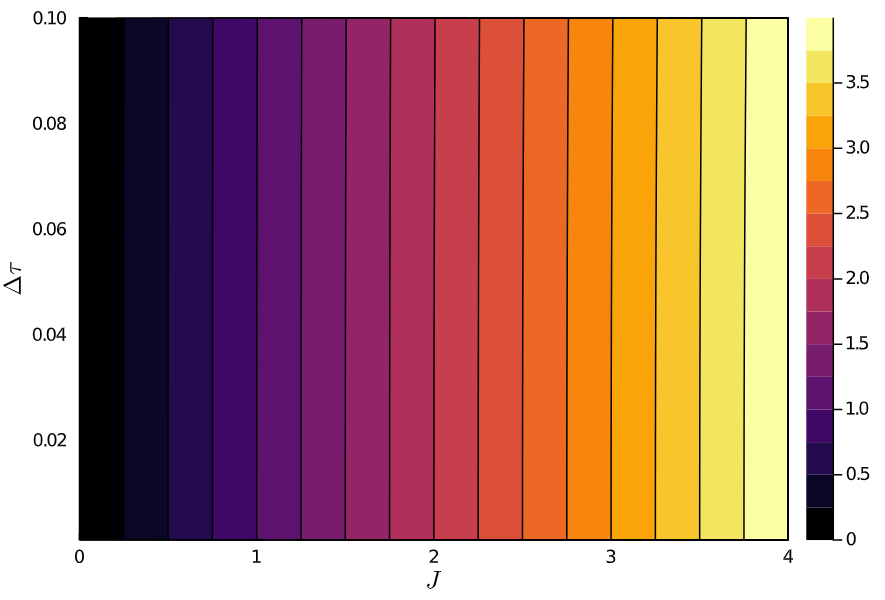
\includegraphics[width=\textwidth]{montecarlo/ratio-h=1.PNG}
        \subcaption{$h = 1$}
    \end{subfigure}
    \begin{subfigure}{0.48\textwidth}
        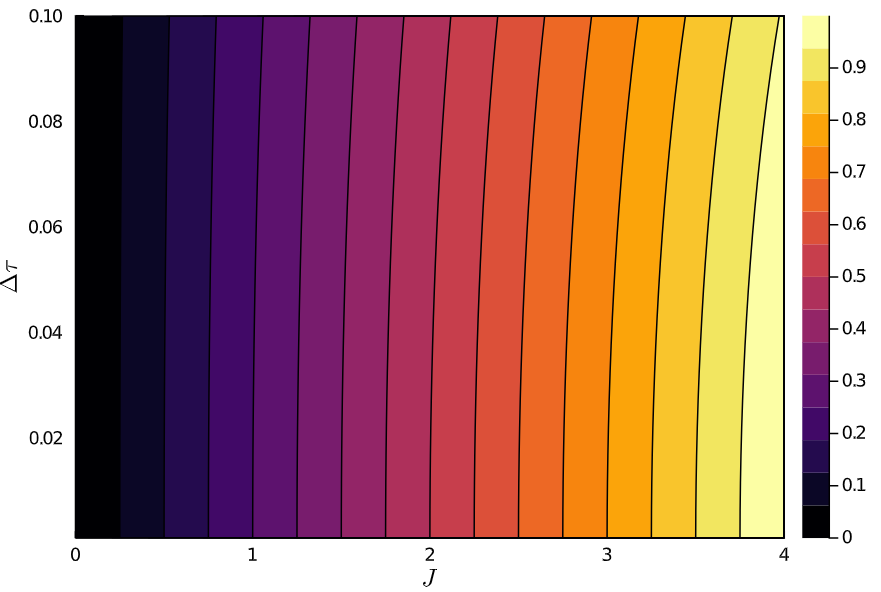
\includegraphics[width=\textwidth]{montecarlo/ratio-h=4.PNG}
        \subcaption{$h = 4$}
    \end{subfigure}
    \caption{$J_{xy} / J_\tau$ under different $h$. 
    It can be seen that \eqref{eq:cim-from-tfim} is highly anisotropic for a large range of $J$.
    Contour lines in (a) are straight, indicating that the discrete path integral works well even with large $\Delta \tau$, 
    while contour lines in (b) are distorted, requiring us to use $\Delta \tau$ that is small enough.}
    \label{fig:jxy-jtau-ratio}
\end{figure}

It should be noted that \eqref{eq:cim-from-tfim} may be highly anisotropic between time and space, 
which can be observed in \prettyref{fig:jxy-jtau-ratio}.
Another fact that can be read from \prettyref{fig:jxy-jtau-ratio} is that for large $h$ $\Delta \tau$ should be smaller to keep the same accuracy.
The larger $h$ is, the stronger the quantum fluctuation is, 
and with strong quantum fluctuation $\Delta \tau$ must be small enough to accurately track the time evolution.

\subsubsection{Cluster update algorithm along the temporal direction}

The anisotropic feature of \eqref{eq:cim-from-tfim} is tackled in \cite{Blte2002}.

We did a benchmark of our algorithm with data provided in \cite{Friedman_1978}.

\subsubsection{Worm algorithm for 2D \tfim}

Another way to simulate 2D \tfim is described in \cite{Huang_2020}.
We do the following (canonical) substitution
\begin{equation}
    \sigma_{\vb*{i}}^x \longrightarrow - \sigma^z_{\vb*{i}}, \quad \sigma_{\vb*{i}}^z \longrightarrow - \sigma^x_{\vb*{i}}, \quad \sigma^y_{\vb*{i}} \longrightarrow - \sigma^y_{\vb*{i}}
\end{equation}
in \eqref{eq:tfim-hamiltonian}, and obtain
\begin{equation}
    H = - J \sum_{\pair{\vb*{i}, \vb*{j}}} \sigma^x_{\vb*{i}} \sigma^x_{\vb*{j}} - h \sum_{\vb*{i}} \sigma^z_{\vb*{i}}.
    \label{eq:tfim-string-form}
\end{equation}
which can be viewed as a string-net model, where the $\sum \sigma^z$ term is string tension term and the other term is the string kinetic term.
The ends of a $\sigma^z$ string are two sites on which $\sigma^z = -1$, as opposed to the ``vacuum'' case where $\sigma^z = 1$.
We define the ladder operators in the standard way
\begin{equation}
    \sigma^\pm_{\vb*{i}} = \frac{\sigma^x_{\vb*{i}} \pm \ii \sigma^y_{\vb*{i}}}{2},
\end{equation}
then \eqref{eq:tfim-string-form} turns into
\begin{equation}
    H = - J \sum_{\pair{\vb*{i}, \vb*{j}}} (\sigma^+_{\vb*{i}} \sigma^-_{\vb*{j}} + \sigma^+_{\vb*{i}} \sigma^+_{\vb*{j}} + \text{h.c.}) - h \sum_{\vb*{i}} \sigma_{\vb*{i}}^z,
    \label{eq:tfim-string-fragments}
\end{equation}
which can also be rewrite into one of hardcore boson model.

\begin{figure}
    \centering
    \begin{subfigure}{0.48\textwidth}
        

\tikzset{every picture/.style={line width=0.75pt}} %set default line width to 0.75pt        

\begin{tikzpicture}[x=0.75pt,y=0.75pt,yscale=-1,xscale=1]
%uncomment if require: \path (0,300); %set diagram left start at 0, and has height of 300

%Straight Lines [id:da1344701610921304] 
\draw    (109.5,114) -- (151.5,114) ;
\draw [shift={(130.5,114)}, rotate = 0] [color={rgb, 255:red, 0; green, 0; blue, 0 }  ][fill={rgb, 255:red, 0; green, 0; blue, 0 }  ][line width=0.75]      (0, 0) circle [x radius= 3.35, y radius= 3.35]   ;
%Straight Lines [id:da9715159999125871] 
\draw    (151.5,114) -- (193.5,114) ;
\draw [shift={(172.5,114)}, rotate = 360] [color={rgb, 255:red, 0; green, 0; blue, 0 }  ][fill={rgb, 255:red, 0; green, 0; blue, 0 }  ][line width=0.75]      (0, 0) circle [x radius= 3.35, y radius= 3.35]   ;
%Straight Lines [id:da15007078493820525] 
\draw    (193.5,114) -- (235.5,114) ;
\draw [shift={(214.5,114)}, rotate = 0] [color={rgb, 255:red, 0; green, 0; blue, 0 }  ][fill={rgb, 255:red, 0; green, 0; blue, 0 }  ][line width=0.75]      (0, 0) circle [x radius= 3.35, y radius= 3.35]   ;
%Straight Lines [id:da4399718858764743] 
\draw    (235.5,114) -- (277.5,114) ;
\draw [shift={(256.5,114)}, rotate = 0] [color={rgb, 255:red, 0; green, 0; blue, 0 }  ][fill={rgb, 255:red, 0; green, 0; blue, 0 }  ][line width=0.75]      (0, 0) circle [x radius= 3.35, y radius= 3.35]   ;
%Straight Lines [id:da1043440459699756] 
\draw    (277.5,114) -- (319.5,114) ;
\draw [shift={(298.5,114)}, rotate = 0] [color={rgb, 255:red, 0; green, 0; blue, 0 }  ][fill={rgb, 255:red, 0; green, 0; blue, 0 }  ][line width=0.75]      (0, 0) circle [x radius= 3.35, y radius= 3.35]   ;
%Straight Lines [id:da6859888870749196] 
\draw    (109.5,179) -- (151.5,179) ;
\draw [shift={(130.5,179)}, rotate = 0] [color={rgb, 255:red, 0; green, 0; blue, 0 }  ][fill={rgb, 255:red, 0; green, 0; blue, 0 }  ][line width=0.75]      (0, 0) circle [x radius= 3.35, y radius= 3.35]   ;
%Straight Lines [id:da1061116367771815] 
\draw    (151.5,179) -- (193.5,179) ;
\draw [shift={(172.5,179)}, rotate = 0] [color={rgb, 255:red, 0; green, 0; blue, 0 }  ][fill={rgb, 255:red, 0; green, 0; blue, 0 }  ][line width=0.75]      (0, 0) circle [x radius= 3.35, y radius= 3.35]   ;
%Straight Lines [id:da597050925918384] 
\draw    (193.5,179) -- (235.5,179) ;
\draw [shift={(214.5,179)}, rotate = 0] [color={rgb, 255:red, 0; green, 0; blue, 0 }  ][fill={rgb, 255:red, 0; green, 0; blue, 0 }  ][line width=0.75]      (0, 0) circle [x radius= 3.35, y radius= 3.35]   ;
%Straight Lines [id:da6334703126215693] 
\draw    (235.5,179) -- (277.5,179) ;
\draw [shift={(256.5,179)}, rotate = 0] [color={rgb, 255:red, 0; green, 0; blue, 0 }  ][fill={rgb, 255:red, 0; green, 0; blue, 0 }  ][line width=0.75]      (0, 0) circle [x radius= 3.35, y radius= 3.35]   ;
%Straight Lines [id:da18416334215363417] 
\draw    (277.5,179) -- (319.5,179) ;
\draw [shift={(298.5,179)}, rotate = 0] [color={rgb, 255:red, 0; green, 0; blue, 0 }  ][fill={rgb, 255:red, 0; green, 0; blue, 0 }  ][line width=0.75]      (0, 0) circle [x radius= 3.35, y radius= 3.35]   ;
%Straight Lines [id:da6013951907749349] 
\draw [color={rgb, 255:red, 208; green, 2; blue, 27 }  ,draw opacity=0.39 ]   (130.5,189.5) -- (130.5,168.5) -- (130.5,161.5) ;
\draw [shift={(130.5,159.5)}, rotate = 450] [fill={rgb, 255:red, 208; green, 2; blue, 27 }  ,fill opacity=0.39 ][line width=0.08]  [draw opacity=0] (12,-3) -- (0,0) -- (12,3) -- cycle    ;
%Straight Lines [id:da9234979061788491] 
\draw [color={rgb, 255:red, 208; green, 2; blue, 27 }  ,draw opacity=0.39 ]   (172.5,189.5) -- (172.5,168.5) -- (172.5,161.5) ;
\draw [shift={(172.5,159.5)}, rotate = 450] [fill={rgb, 255:red, 208; green, 2; blue, 27 }  ,fill opacity=0.39 ][line width=0.08]  [draw opacity=0] (12,-3) -- (0,0) -- (12,3) -- cycle    ;
%Straight Lines [id:da8201433352928262] 
\draw [color={rgb, 255:red, 208; green, 2; blue, 27 }  ,draw opacity=0.39 ]   (214.5,189.5) -- (214.5,168.5) -- (214.5,161.5) ;
\draw [shift={(214.5,159.5)}, rotate = 450] [fill={rgb, 255:red, 208; green, 2; blue, 27 }  ,fill opacity=0.39 ][line width=0.08]  [draw opacity=0] (12,-3) -- (0,0) -- (12,3) -- cycle    ;
%Straight Lines [id:da8706270770680999] 
\draw [color={rgb, 255:red, 208; green, 2; blue, 27 }  ,draw opacity=0.39 ]   (256.5,189.5) -- (256.5,168.5) -- (256.5,161.5) ;
\draw [shift={(256.5,159.5)}, rotate = 450] [fill={rgb, 255:red, 208; green, 2; blue, 27 }  ,fill opacity=0.39 ][line width=0.08]  [draw opacity=0] (12,-3) -- (0,0) -- (12,3) -- cycle    ;
%Straight Lines [id:da79494202599026] 
\draw [color={rgb, 255:red, 208; green, 2; blue, 27 }  ,draw opacity=0.39 ]   (298.5,189.5) -- (298.5,168.5) -- (298.5,161.5) ;
\draw [shift={(298.5,159.5)}, rotate = 450] [fill={rgb, 255:red, 208; green, 2; blue, 27 }  ,fill opacity=0.39 ][line width=0.08]  [draw opacity=0] (12,-3) -- (0,0) -- (12,3) -- cycle    ;
%Straight Lines [id:da759606249190288] 
\draw [color={rgb, 255:red, 208; green, 2; blue, 27 }  ,draw opacity=0.39 ]   (130.5,124.5) -- (130.5,103.5) -- (130.5,96.5) ;
\draw [shift={(130.5,94.5)}, rotate = 450] [fill={rgb, 255:red, 208; green, 2; blue, 27 }  ,fill opacity=0.39 ][line width=0.08]  [draw opacity=0] (12,-3) -- (0,0) -- (12,3) -- cycle    ;
%Straight Lines [id:da8367215263190646] 
\draw [color={rgb, 255:red, 208; green, 2; blue, 27 }  ,draw opacity=0.39 ]   (298.5,124.5) -- (298.5,103.5) -- (298.5,96.5) ;
\draw [shift={(298.5,94.5)}, rotate = 450] [fill={rgb, 255:red, 208; green, 2; blue, 27 }  ,fill opacity=0.39 ][line width=0.08]  [draw opacity=0] (12,-3) -- (0,0) -- (12,3) -- cycle    ;
%Straight Lines [id:da2428035707775147] 
\draw [color={rgb, 255:red, 245; green, 166; blue, 35 }  ,draw opacity=1 ][line width=1.5]    (172.5,114) -- (214.5,114) ;
%Straight Lines [id:da8600979922109195] 
\draw [color={rgb, 255:red, 208; green, 2; blue, 27 }  ,draw opacity=1 ]   (172.5,103.5) -- (172.5,124.5) -- (172.5,131.5) ;
\draw [shift={(172.5,133.5)}, rotate = 270] [fill={rgb, 255:red, 208; green, 2; blue, 27 }  ,fill opacity=1 ][line width=0.08]  [draw opacity=0] (12,-3) -- (0,0) -- (12,3) -- cycle    ;
%Straight Lines [id:da09111610716922125] 
\draw [color={rgb, 255:red, 208; green, 2; blue, 27 }  ,draw opacity=1 ]   (214.5,103.5) -- (214.5,124.5) -- (214.5,131.5) ;
\draw [shift={(214.5,133.5)}, rotate = 270] [fill={rgb, 255:red, 208; green, 2; blue, 27 }  ,fill opacity=1 ][line width=0.08]  [draw opacity=0] (12,-3) -- (0,0) -- (12,3) -- cycle    ;
%Straight Lines [id:da26498774370531053] 
\draw [color={rgb, 255:red, 208; green, 2; blue, 27 }  ,draw opacity=0.39 ]   (256.5,124.5) -- (256.5,103.5) -- (256.5,96.5) ;
\draw [shift={(256.5,94.5)}, rotate = 450] [fill={rgb, 255:red, 208; green, 2; blue, 27 }  ,fill opacity=0.39 ][line width=0.08]  [draw opacity=0] (12,-3) -- (0,0) -- (12,3) -- cycle    ;

% Text Node
\draw (107.5,179) node [anchor=east] [inner sep=0.75pt]    {$\tau $};
% Text Node
\draw (107.5,114) node [anchor=east] [inner sep=0.75pt]    {$\tau +\Delta \tau $};


\end{tikzpicture}

        \subcaption{}
    \end{subfigure}
    \begin{subfigure}{0.48\textwidth}
        

\tikzset{every picture/.style={line width=0.75pt}} %set default line width to 0.75pt        

\begin{tikzpicture}[x=0.75pt,y=0.75pt,yscale=-1,xscale=1]
%uncomment if require: \path (0,300); %set diagram left start at 0, and has height of 300

%Straight Lines [id:da8927644578577054] 
\draw    (129.5,134) -- (171.5,134) ;
\draw [shift={(150.5,134)}, rotate = 0] [color={rgb, 255:red, 0; green, 0; blue, 0 }  ][fill={rgb, 255:red, 0; green, 0; blue, 0 }  ][line width=0.75]      (0, 0) circle [x radius= 3.35, y radius= 3.35]   ;
%Straight Lines [id:da6996734855769833] 
\draw    (171.5,134) -- (213.5,134) ;
\draw [shift={(192.5,134)}, rotate = 0] [color={rgb, 255:red, 0; green, 0; blue, 0 }  ][fill={rgb, 255:red, 0; green, 0; blue, 0 }  ][line width=0.75]      (0, 0) circle [x radius= 3.35, y radius= 3.35]   ;
%Straight Lines [id:da4748034691973022] 
\draw    (213.5,134) -- (255.5,134) ;
\draw [shift={(234.5,134)}, rotate = 0] [color={rgb, 255:red, 0; green, 0; blue, 0 }  ][fill={rgb, 255:red, 0; green, 0; blue, 0 }  ][line width=0.75]      (0, 0) circle [x radius= 3.35, y radius= 3.35]   ;
%Straight Lines [id:da16666577767236368] 
\draw    (255.5,134) -- (297.5,134) ;
\draw [shift={(276.5,134)}, rotate = 0] [color={rgb, 255:red, 0; green, 0; blue, 0 }  ][fill={rgb, 255:red, 0; green, 0; blue, 0 }  ][line width=0.75]      (0, 0) circle [x radius= 3.35, y radius= 3.35]   ;
%Straight Lines [id:da976661403256808] 
\draw    (297.5,134) -- (339.5,134) ;
\draw [shift={(318.5,134)}, rotate = 0] [color={rgb, 255:red, 0; green, 0; blue, 0 }  ][fill={rgb, 255:red, 0; green, 0; blue, 0 }  ][line width=0.75]      (0, 0) circle [x radius= 3.35, y radius= 3.35]   ;
%Straight Lines [id:da06650182682423256] 
\draw    (129.5,199) -- (171.5,199) ;
\draw [shift={(150.5,199)}, rotate = 0] [color={rgb, 255:red, 0; green, 0; blue, 0 }  ][fill={rgb, 255:red, 0; green, 0; blue, 0 }  ][line width=0.75]      (0, 0) circle [x radius= 3.35, y radius= 3.35]   ;
%Straight Lines [id:da753042837501475] 
\draw    (171.5,199) -- (213.5,199) ;
\draw [shift={(192.5,199)}, rotate = 0] [color={rgb, 255:red, 0; green, 0; blue, 0 }  ][fill={rgb, 255:red, 0; green, 0; blue, 0 }  ][line width=0.75]      (0, 0) circle [x radius= 3.35, y radius= 3.35]   ;
%Straight Lines [id:da2592926712827657] 
\draw    (213.5,199) -- (255.5,199) ;
\draw [shift={(234.5,199)}, rotate = 0] [color={rgb, 255:red, 0; green, 0; blue, 0 }  ][fill={rgb, 255:red, 0; green, 0; blue, 0 }  ][line width=0.75]      (0, 0) circle [x radius= 3.35, y radius= 3.35]   ;
%Straight Lines [id:da4452229679373816] 
\draw    (255.5,199) -- (297.5,199) ;
\draw [shift={(276.5,199)}, rotate = 0] [color={rgb, 255:red, 0; green, 0; blue, 0 }  ][fill={rgb, 255:red, 0; green, 0; blue, 0 }  ][line width=0.75]      (0, 0) circle [x radius= 3.35, y radius= 3.35]   ;
%Straight Lines [id:da3665763653349059] 
\draw    (297.5,199) -- (339.5,199) ;
\draw [shift={(318.5,199)}, rotate = 0] [color={rgb, 255:red, 0; green, 0; blue, 0 }  ][fill={rgb, 255:red, 0; green, 0; blue, 0 }  ][line width=0.75]      (0, 0) circle [x radius= 3.35, y radius= 3.35]   ;
%Straight Lines [id:da8998940933719315] 
\draw [color={rgb, 255:red, 208; green, 2; blue, 27 }  ,draw opacity=0.39 ]   (150.5,209.5) -- (150.5,188.5) -- (150.5,181.5) ;
\draw [shift={(150.5,179.5)}, rotate = 450] [fill={rgb, 255:red, 208; green, 2; blue, 27 }  ,fill opacity=0.39 ][line width=0.08]  [draw opacity=0] (12,-3) -- (0,0) -- (12,3) -- cycle    ;
%Straight Lines [id:da26865841249392153] 
\draw [color={rgb, 255:red, 208; green, 2; blue, 27 }  ,draw opacity=0.39 ]   (192.5,209.5) -- (192.5,188.5) -- (192.5,181.5) ;
\draw [shift={(192.5,179.5)}, rotate = 450] [fill={rgb, 255:red, 208; green, 2; blue, 27 }  ,fill opacity=0.39 ][line width=0.08]  [draw opacity=0] (12,-3) -- (0,0) -- (12,3) -- cycle    ;
%Straight Lines [id:da27930114202599987] 
\draw [color={rgb, 255:red, 208; green, 2; blue, 27 }  ,draw opacity=0.39 ]   (150.5,144.5) -- (150.5,123.5) -- (150.5,116.5) ;
\draw [shift={(150.5,114.5)}, rotate = 450] [fill={rgb, 255:red, 208; green, 2; blue, 27 }  ,fill opacity=0.39 ][line width=0.08]  [draw opacity=0] (12,-3) -- (0,0) -- (12,3) -- cycle    ;
%Straight Lines [id:da17999132919076666] 
\draw [color={rgb, 255:red, 248; green, 231; blue, 28 }  ,draw opacity=1 ][line width=1.5]    (192.5,134) -- (339.5,134) ;
%Straight Lines [id:da8879404302074527] 
\draw [color={rgb, 255:red, 248; green, 231; blue, 28 }  ,draw opacity=1 ][line width=1.5]    (234.5,199) -- (339.5,199) ;
%Straight Lines [id:da7232037795096793] 
\draw [color={rgb, 255:red, 208; green, 2; blue, 27 }  ,draw opacity=0.39 ]   (276.5,144.5) -- (276.5,123.5) -- (276.5,116.5) ;
\draw [shift={(276.5,114.5)}, rotate = 450] [fill={rgb, 255:red, 208; green, 2; blue, 27 }  ,fill opacity=0.39 ][line width=0.08]  [draw opacity=0] (12,-3) -- (0,0) -- (12,3) -- cycle    ;
%Straight Lines [id:da9040416544728251] 
\draw [color={rgb, 255:red, 208; green, 2; blue, 27 }  ,draw opacity=0.39 ]   (234.5,144.5) -- (234.5,123.5) -- (234.5,116.5) ;
\draw [shift={(234.5,114.5)}, rotate = 450] [fill={rgb, 255:red, 208; green, 2; blue, 27 }  ,fill opacity=0.39 ][line width=0.08]  [draw opacity=0] (12,-3) -- (0,0) -- (12,3) -- cycle    ;
%Straight Lines [id:da10156711700094467] 
\draw [color={rgb, 255:red, 208; green, 2; blue, 27 }  ,draw opacity=0.39 ]   (318.5,144.5) -- (318.5,123.5) -- (318.5,116.5) ;
\draw [shift={(318.5,114.5)}, rotate = 450] [fill={rgb, 255:red, 208; green, 2; blue, 27 }  ,fill opacity=0.39 ][line width=0.08]  [draw opacity=0] (12,-3) -- (0,0) -- (12,3) -- cycle    ;
%Straight Lines [id:da1333991139019972] 
\draw [color={rgb, 255:red, 208; green, 2; blue, 27 }  ,draw opacity=0.39 ]   (276.5,209.5) -- (276.5,188.5) -- (276.5,181.5) ;
\draw [shift={(276.5,179.5)}, rotate = 450] [fill={rgb, 255:red, 208; green, 2; blue, 27 }  ,fill opacity=0.39 ][line width=0.08]  [draw opacity=0] (12,-3) -- (0,0) -- (12,3) -- cycle    ;
%Straight Lines [id:da6834741570503935] 
\draw [color={rgb, 255:red, 208; green, 2; blue, 27 }  ,draw opacity=0.39 ]   (318.5,209.5) -- (318.5,188.5) -- (318.5,181.5) ;
\draw [shift={(318.5,179.5)}, rotate = 450] [fill={rgb, 255:red, 208; green, 2; blue, 27 }  ,fill opacity=0.39 ][line width=0.08]  [draw opacity=0] (12,-3) -- (0,0) -- (12,3) -- cycle    ;
%Straight Lines [id:da30915794511383266] 
\draw [color={rgb, 255:red, 245; green, 166; blue, 35 }  ,draw opacity=1 ][line width=1.5]    (192.5,134) -- (234.5,134) ;
%Straight Lines [id:da9718948895733661] 
\draw [color={rgb, 255:red, 208; green, 2; blue, 27 }  ,draw opacity=1 ]   (192.5,123.5) -- (192.5,144.5) -- (192.5,151.5) ;
\draw [shift={(192.5,153.5)}, rotate = 270] [fill={rgb, 255:red, 208; green, 2; blue, 27 }  ,fill opacity=1 ][line width=0.08]  [draw opacity=0] (12,-3) -- (0,0) -- (12,3) -- cycle    ;
%Straight Lines [id:da5074022584810736] 
\draw [color={rgb, 255:red, 208; green, 2; blue, 27 }  ,draw opacity=1 ]   (234.5,188.5) -- (234.5,209.5) -- (234.5,216.5) ;
\draw [shift={(234.5,218.5)}, rotate = 270] [fill={rgb, 255:red, 208; green, 2; blue, 27 }  ,fill opacity=1 ][line width=0.08]  [draw opacity=0] (12,-3) -- (0,0) -- (12,3) -- cycle    ;

% Text Node
\draw (127.5,199) node [anchor=east] [inner sep=0.75pt]    {$\tau $};
% Text Node
\draw (127.5,134) node [anchor=east] [inner sep=0.75pt]    {$\tau +\Delta \tau $};


\end{tikzpicture}

        \subcaption{}
    \end{subfigure}
    \caption{String fragments provided in \eqref{eq:tfim-string-fragments}. 
    (a) corresponds to the $\sigma^+ \sigma^+$ term, where a minimal string is created out of nothing, 
    or in other words, two magnons are created out of nothing.
    (b) corresponds to the $\sigma^+ \sigma^-$ term, which extends an existing string, 
    or in other words, a magnon is moved to its nearest neighbor. 
    The time inverse of (a) and (b) can be easily found, which are annihilation of a minimal string and shortening an existing string, correspondingly.}
    \label{fig:tfim-string-fragments}
\end{figure}

The $\sigma^z$ strings can expand and shrink, and their ends can hop from one site to its neighbors, 
according to the first four terms in the Hamiltonian, which are factories of string fragments.
This is visualize in \prettyref{fig:tfim-string-fragments}.
It should be noted that the $\sigma^+ \sigma^+$ term only applies to vacuum, or otherwise it just returns zero.
Likewise, the $\sigma^+ \sigma^-$ term only applies to existing strings, or otherwise it just returns zero.
Two or more minimal strings can be created at the same time, 
so effectively, a prolonged string can be generated from vacuum in just one time step.
As a result, the field configuration used in the path integral is something like this: 
a string is created, and then distorted, and finally annihilated.
So each field configuration used in the path integral is a set of \emph{closed} strings or loops, 
which are just \emph{world lines} of magnons, as is depicted in \prettyref{fig:tfim-worldline}.
We name the $\sigma^+ \sigma^+ + \text{h.c.}$ terms as \concept{pairing}, the $\sigma^+ \sigma^- + \text{h.c.}$ terms \concept{hopping}.

\begin{figure}
    \centering
    

\tikzset{every picture/.style={line width=0.75pt}} %set default line width to 0.75pt        

\begin{tikzpicture}[x=0.75pt,y=0.75pt,yscale=-1,xscale=1]
%uncomment if require: \path (0,300); %set diagram left start at 0, and has height of 300

%Shape: Square [id:dp4479686036486705] 
\draw  [color={rgb, 255:red, 0; green, 0; blue, 0 }  ,draw opacity=0.25 ] (193.33,65.33) -- (227.67,65.33) -- (227.67,99.67) -- (193.33,99.67) -- cycle ;
%Shape: Square [id:dp21218390506026652] 
\draw  [color={rgb, 255:red, 0; green, 0; blue, 0 }  ,draw opacity=0.25 ] (262,65.33) -- (296.33,65.33) -- (296.33,99.67) -- (262,99.67) -- cycle ;
%Shape: Square [id:dp7298786133483419] 
\draw  [color={rgb, 255:red, 0; green, 0; blue, 0 }  ,draw opacity=0.25 ] (296.33,65.33) -- (330.67,65.33) -- (330.67,99.67) -- (296.33,99.67) -- cycle ;
%Shape: Square [id:dp9020944166766589] 
\draw  [color={rgb, 255:red, 0; green, 0; blue, 0 }  ,draw opacity=0.25 ] (330.67,65.33) -- (365,65.33) -- (365,99.67) -- (330.67,99.67) -- cycle ;
%Shape: Square [id:dp4923829385472134] 
\draw  [color={rgb, 255:red, 0; green, 0; blue, 0 }  ,draw opacity=0.25 ] (365,65.33) -- (399.33,65.33) -- (399.33,99.67) -- (365,99.67) -- cycle ;
%Shape: Square [id:dp571238050965464] 
\draw  [color={rgb, 255:red, 0; green, 0; blue, 0 }  ,draw opacity=0.25 ] (399.33,65.33) -- (433.67,65.33) -- (433.67,99.67) -- (399.33,99.67) -- cycle ;
%Shape: Square [id:dp8322680589990272] 
\draw  [color={rgb, 255:red, 0; green, 0; blue, 0 }  ,draw opacity=0.25 ] (193.33,99.67) -- (227.67,99.67) -- (227.67,134) -- (193.33,134) -- cycle ;
%Shape: Square [id:dp6332973434519487] 
\draw  [color={rgb, 255:red, 0; green, 0; blue, 0 }  ,draw opacity=0.25 ] (262,99.67) -- (296.33,99.67) -- (296.33,134) -- (262,134) -- cycle ;
%Shape: Square [id:dp9018510066958652] 
\draw  [color={rgb, 255:red, 0; green, 0; blue, 0 }  ,draw opacity=0.25 ] (296.33,99.67) -- (330.67,99.67) -- (330.67,134) -- (296.33,134) -- cycle ;
%Shape: Square [id:dp921202264296372] 
\draw  [color={rgb, 255:red, 0; green, 0; blue, 0 }  ,draw opacity=0.25 ] (330.67,99.67) -- (365,99.67) -- (365,134) -- (330.67,134) -- cycle ;
%Shape: Square [id:dp9707434128776609] 
\draw  [color={rgb, 255:red, 0; green, 0; blue, 0 }  ,draw opacity=0.25 ] (365,99.67) -- (399.33,99.67) -- (399.33,134) -- (365,134) -- cycle ;
%Shape: Square [id:dp39460938718614913] 
\draw  [color={rgb, 255:red, 0; green, 0; blue, 0 }  ,draw opacity=0.25 ] (399.33,99.67) -- (433.67,99.67) -- (433.67,134) -- (399.33,134) -- cycle ;
%Shape: Square [id:dp04755070663903571] 
\draw  [color={rgb, 255:red, 0; green, 0; blue, 0 }  ,draw opacity=0.25 ] (193.33,134) -- (227.67,134) -- (227.67,168.33) -- (193.33,168.33) -- cycle ;
%Shape: Square [id:dp22524145985782518] 
\draw  [color={rgb, 255:red, 0; green, 0; blue, 0 }  ,draw opacity=0.25 ] (262,134) -- (296.33,134) -- (296.33,168.33) -- (262,168.33) -- cycle ;
%Shape: Square [id:dp1559089508020295] 
\draw  [color={rgb, 255:red, 0; green, 0; blue, 0 }  ,draw opacity=0.25 ] (296.33,134) -- (330.67,134) -- (330.67,168.33) -- (296.33,168.33) -- cycle ;
%Shape: Square [id:dp015395655151661858] 
\draw  [color={rgb, 255:red, 0; green, 0; blue, 0 }  ,draw opacity=0.25 ] (330.67,134) -- (365,134) -- (365,168.33) -- (330.67,168.33) -- cycle ;
%Shape: Square [id:dp006880897031339428] 
\draw  [color={rgb, 255:red, 0; green, 0; blue, 0 }  ,draw opacity=0.25 ] (365,134) -- (399.33,134) -- (399.33,168.33) -- (365,168.33) -- cycle ;
%Shape: Square [id:dp37020949877483966] 
\draw  [color={rgb, 255:red, 0; green, 0; blue, 0 }  ,draw opacity=0.25 ] (399.33,134) -- (433.67,134) -- (433.67,168.33) -- (399.33,168.33) -- cycle ;
%Shape: Square [id:dp3346562733387046] 
\draw  [color={rgb, 255:red, 0; green, 0; blue, 0 }  ,draw opacity=0.25 ] (193.33,168.33) -- (227.67,168.33) -- (227.67,202.67) -- (193.33,202.67) -- cycle ;
%Shape: Square [id:dp6204348087107601] 
\draw  [color={rgb, 255:red, 0; green, 0; blue, 0 }  ,draw opacity=0.25 ] (262,168.33) -- (296.33,168.33) -- (296.33,202.67) -- (262,202.67) -- cycle ;
%Shape: Square [id:dp7038254138703566] 
\draw  [color={rgb, 255:red, 0; green, 0; blue, 0 }  ,draw opacity=0.25 ] (296.33,168.33) -- (330.67,168.33) -- (330.67,202.67) -- (296.33,202.67) -- cycle ;
%Shape: Square [id:dp48275605655503107] 
\draw  [color={rgb, 255:red, 0; green, 0; blue, 0 }  ,draw opacity=0.25 ] (330.67,168.33) -- (365,168.33) -- (365,202.67) -- (330.67,202.67) -- cycle ;
%Shape: Square [id:dp7521992992410951] 
\draw  [color={rgb, 255:red, 0; green, 0; blue, 0 }  ,draw opacity=0.25 ] (365,168.33) -- (399.33,168.33) -- (399.33,202.67) -- (365,202.67) -- cycle ;
%Shape: Square [id:dp9422129738109646] 
\draw  [color={rgb, 255:red, 0; green, 0; blue, 0 }  ,draw opacity=0.25 ] (399.33,168.33) -- (433.67,168.33) -- (433.67,202.67) -- (399.33,202.67) -- cycle ;
%Straight Lines [id:da5443524763391978] 
\draw [color={rgb, 255:red, 245; green, 166; blue, 35 }  ,draw opacity=1 ][line width=3]    (296.33,168.33) -- (330.67,168.33) ;
%Straight Lines [id:da9232682389537956] 
\draw [color={rgb, 255:red, 245; green, 166; blue, 35 }  ,draw opacity=1 ][line width=3]    (330.67,168.33) -- (365,168.33) ;
%Straight Lines [id:da938291222599466] 
\draw [color={rgb, 255:red, 245; green, 166; blue, 35 }  ,draw opacity=1 ][line width=3]    (262,134) -- (296.33,134) ;
%Straight Lines [id:da18896587427258793] 
\draw [color={rgb, 255:red, 0; green, 0; blue, 0 }  ,draw opacity=1 ]   (296.33,202.67) -- (296.33,168.33) ;
%Straight Lines [id:da34056637521076927] 
\draw [color={rgb, 255:red, 245; green, 166; blue, 35 }  ,draw opacity=1 ][line width=3]    (296.33,202.67) -- (330.67,202.67) ;
%Straight Lines [id:da9328634543619851] 
\draw [color={rgb, 255:red, 0; green, 0; blue, 0 }  ,draw opacity=1 ][line width=0.75]    (330.67,202.67) -- (296.33,202.67) ;
%Straight Lines [id:da21252429371670356] 
\draw [color={rgb, 255:red, 245; green, 166; blue, 35 }  ,draw opacity=1 ][line width=3]    (296.33,134) -- (330.67,134) ;
%Straight Lines [id:da8347591732615751] 
\draw [color={rgb, 255:red, 0; green, 0; blue, 0 }  ,draw opacity=1 ]   (330.67,202.67) -- (365,168.33) ;
%Straight Lines [id:da5163542822207372] 
\draw [color={rgb, 255:red, 0; green, 0; blue, 0 }  ,draw opacity=1 ]   (262,134) -- (296.33,168.33) ;
%Straight Lines [id:da5507379443435076] 
\draw [color={rgb, 255:red, 245; green, 166; blue, 35 }  ,draw opacity=1 ][line width=3]    (330.67,134) -- (365,134) ;
%Straight Lines [id:da6737757999979572] 
\draw [color={rgb, 255:red, 0; green, 0; blue, 0 }  ,draw opacity=1 ]   (365,134) -- (365,168.33) ;
%Straight Lines [id:da31007406949322824] 
\draw [color={rgb, 255:red, 0; green, 0; blue, 0 }  ,draw opacity=1 ]   (330.67,99.67) -- (365,134) ;
%Straight Lines [id:da8269194573500334] 
\draw [color={rgb, 255:red, 0; green, 0; blue, 0 }  ,draw opacity=1 ]   (262,134) -- (296.33,99.67) ;
%Straight Lines [id:da09615146724644075] 
\draw [color={rgb, 255:red, 245; green, 166; blue, 35 }  ,draw opacity=1 ][line width=3]    (296.33,99.67) -- (330.67,99.67) ;
%Straight Lines [id:da8877325558928841] 
\draw [color={rgb, 255:red, 245; green, 166; blue, 35 }  ,draw opacity=1 ][line width=3]    (296.33,65.33) -- (330.67,65.33) ;
%Straight Lines [id:da21887514563166555] 
\draw [color={rgb, 255:red, 0; green, 0; blue, 0 }  ,draw opacity=1 ]   (296.33,65.33) -- (296.33,99.67) ;
%Straight Lines [id:da651570592828693] 
\draw [color={rgb, 255:red, 0; green, 0; blue, 0 }  ,draw opacity=1 ]   (330.67,65.33) -- (330.67,99.67) ;
%Straight Lines [id:da6720953717549225] 
\draw [color={rgb, 255:red, 0; green, 0; blue, 0 }  ,draw opacity=1 ]   (296.33,65.33) -- (330.67,65.33) ;
%Shape: Square [id:dp4447455564826208] 
\draw  [color={rgb, 255:red, 0; green, 0; blue, 0 }  ,draw opacity=0.25 ] (433.33,65.33) -- (467.67,65.33) -- (467.67,99.67) -- (433.33,99.67) -- cycle ;
%Shape: Square [id:dp01696912357284619] 
\draw  [color={rgb, 255:red, 0; green, 0; blue, 0 }  ,draw opacity=0.25 ] (433.33,99.67) -- (467.67,99.67) -- (467.67,134) -- (433.33,134) -- cycle ;
%Shape: Square [id:dp785500733451779] 
\draw  [color={rgb, 255:red, 0; green, 0; blue, 0 }  ,draw opacity=0.25 ] (433.33,134) -- (467.67,134) -- (467.67,168.33) -- (433.33,168.33) -- cycle ;
%Shape: Square [id:dp3881877279757622] 
\draw  [color={rgb, 255:red, 0; green, 0; blue, 0 }  ,draw opacity=0.25 ] (433.33,168.33) -- (467.67,168.33) -- (467.67,202.67) -- (433.33,202.67) -- cycle ;
%Straight Lines [id:da712520317572318] 
\draw [color={rgb, 255:red, 245; green, 166; blue, 35 }  ,draw opacity=1 ][line width=3]    (399.33,168.33) -- (433.67,168.33) ;
%Straight Lines [id:da9645354260827115] 
\draw [color={rgb, 255:red, 245; green, 166; blue, 35 }  ,draw opacity=1 ][line width=3]    (433.67,168.33) -- (468,168.33) ;
%Shape: Square [id:dp7623742030383029] 
\draw  [color={rgb, 255:red, 0; green, 0; blue, 0 }  ,draw opacity=0.25 ] (227.67,65.33) -- (262,65.33) -- (262,99.67) -- (227.67,99.67) -- cycle ;
%Shape: Square [id:dp07948167634805192] 
\draw  [color={rgb, 255:red, 0; green, 0; blue, 0 }  ,draw opacity=0.25 ] (227.67,99.67) -- (262,99.67) -- (262,134) -- (227.67,134) -- cycle ;
%Shape: Square [id:dp44760997867870667] 
\draw  [color={rgb, 255:red, 0; green, 0; blue, 0 }  ,draw opacity=0.25 ] (227.67,134) -- (262,134) -- (262,168.33) -- (227.67,168.33) -- cycle ;
%Shape: Square [id:dp662601805957926] 
\draw  [color={rgb, 255:red, 0; green, 0; blue, 0 }  ,draw opacity=0.25 ] (227.67,168.33) -- (262,168.33) -- (262,202.67) -- (227.67,202.67) -- cycle ;
%Straight Lines [id:da4173560902675957] 
\draw [color={rgb, 255:red, 245; green, 166; blue, 35 }  ,draw opacity=1 ][line width=3]    (399.33,134) -- (433.67,134) ;
%Straight Lines [id:da43255771660550213] 
\draw [color={rgb, 255:red, 245; green, 166; blue, 35 }  ,draw opacity=1 ][line width=3]    (433.33,134) -- (467.67,134) ;
%Straight Lines [id:da14697126917386472] 
\draw [color={rgb, 255:red, 245; green, 166; blue, 35 }  ,draw opacity=1 ][line width=3]    (193.33,134) -- (227.67,134) ;
%Straight Lines [id:da22205181005845276] 
\draw [color={rgb, 255:red, 0; green, 0; blue, 0 }  ,draw opacity=1 ][line width=0.75]    (433.67,168.33) -- (399.33,168.33) ;
%Straight Lines [id:da028878649443297322] 
\draw [color={rgb, 255:red, 0; green, 0; blue, 0 }  ,draw opacity=1 ][line width=0.75]    (468,168.33) -- (433.67,168.33) ;
%Straight Lines [id:da7636823107193544] 
\draw [color={rgb, 255:red, 0; green, 0; blue, 0 }  ,draw opacity=1 ]   (399.33,134) -- (399.33,168.33) ;
%Straight Lines [id:da22639239755641238] 
\draw [color={rgb, 255:red, 0; green, 0; blue, 0 }  ,draw opacity=1 ]   (193.33,168.33) -- (227.67,134) ;
%Straight Lines [id:da32546846917551964] 
\draw [color={rgb, 255:red, 0; green, 0; blue, 0 }  ,draw opacity=1 ][line width=0.75]    (433.33,134) -- (399,134) ;
%Straight Lines [id:da7215867831995155] 
\draw [color={rgb, 255:red, 0; green, 0; blue, 0 }  ,draw opacity=1 ][line width=0.75]    (467.67,134) -- (433.33,134) ;
%Straight Lines [id:da40601923152927566] 
\draw [color={rgb, 255:red, 0; green, 0; blue, 0 }  ,draw opacity=1 ][line width=0.75]    (227.67,134) -- (193.33,134) ;
%Straight Lines [id:da6899140252757279] 
\draw  [dash pattern={on 4.5pt off 4.5pt}]  (193.36,174.51) -- (467.98,174.51) ;
%Shape: Arc [id:dp5045593338100327] 
\draw  [draw opacity=0] (193.36,174.51) .. controls (190.56,174.45) and (188.33,173.09) .. (188.33,171.42) .. controls (188.33,169.76) and (190.55,168.4) .. (193.33,168.33) -- (193.55,171.42) -- cycle ; \draw   (193.36,174.51) .. controls (190.56,174.45) and (188.33,173.09) .. (188.33,171.42) .. controls (188.33,169.76) and (190.55,168.4) .. (193.33,168.33) ;
%Shape: Arc [id:dp39064094085891377] 
\draw  [draw opacity=0] (467.98,174.51) .. controls (470.77,174.45) and (473.01,173.09) .. (473.01,171.42) .. controls (473.01,169.76) and (470.78,168.4) .. (468,168.33) -- (467.78,171.42) -- cycle ; \draw   (467.98,174.51) .. controls (470.77,174.45) and (473.01,173.09) .. (473.01,171.42) .. controls (473.01,169.76) and (470.78,168.4) .. (468,168.33) ;
%Straight Lines [id:da49459459349803203] 
\draw  [dash pattern={on 4.5pt off 4.5pt}]  (192.02,127.85) -- (466.64,127.85) ;
%Shape: Arc [id:dp8741727626593181] 
\draw  [draw opacity=0] (467.67,134) .. controls (470.46,133.94) and (472.69,132.58) .. (472.69,130.91) .. controls (472.69,129.25) and (470.47,127.89) .. (467.69,127.82) -- (467.47,130.91) -- cycle ; \draw   (467.67,134) .. controls (470.46,133.94) and (472.69,132.58) .. (472.69,130.91) .. controls (472.69,129.25) and (470.47,127.89) .. (467.69,127.82) ;
%Shape: Arc [id:dp22681433011423313] 
\draw  [draw opacity=0] (193.04,134.03) .. controls (190.25,133.96) and (188.02,132.6) .. (188.02,130.94) .. controls (188.02,129.27) and (190.24,127.91) .. (193.02,127.85) -- (193.24,130.94) -- cycle ; \draw   (193.04,134.03) .. controls (190.25,133.96) and (188.02,132.6) .. (188.02,130.94) .. controls (188.02,129.27) and (190.24,127.91) .. (193.02,127.85) ;

% Text Node
\draw (168.33,202.67) node [anchor=east] [inner sep=0.75pt]    {$\tau $};
% Text Node
\draw (166.33,168.33) node [anchor=east] [inner sep=0.75pt]    {$\tau +\Delta \tau $};
% Text Node
\draw (168.33,134) node [anchor=east] [inner sep=0.75pt]    {$\tau +2\Delta \tau $};
% Text Node
\draw (168.33,99.67) node [anchor=east] [inner sep=0.75pt]    {$\tau +3\Delta \tau $};
% Text Node
\draw (168.33,65.33) node [anchor=east] [inner sep=0.75pt]    {$\tau +4\Delta \tau $};


\end{tikzpicture}

    \caption{World lines of magnons in a \tfim model, under the periodic boundary condition. Note that a loop can go across the boundary.}
    \label{fig:tfim-worldline}
\end{figure}

Now we write down the partition function in the path integral form.
Suppose there are $m$ time steps. The discrete path integral is 
\begin{equation}
    Z = \sum_{\{\sigma_\tau\}} \mel{\sigma_0}{\ee^{-\Delta \tau H}}{\sigma_\beta} \cdots \mel{\sigma_{2\Delta \tau}}{\ee^{-\Delta \tau H}}{\sigma_{\Delta \tau}} \mel{\sigma_{\Delta \tau}}{\ee^{-\Delta \tau H}}{\sigma_{0}}  
\end{equation}
where $\sigma_\tau$ is an arbitrary configuration in the $\sigma^z$ basis.
We classify $\{\sigma_\tau\}$ first according to the number of pairing and hopping, and denote them as $N_\text{p}$ and $N_\text{h}$, respectively.
The weight of a field configuration with $N_\text{p}$ pairing fragments and $N_\text{h}$ hopping fragments is
\[
    \mel{\sigma_0}{\ee^{-\Delta \tau H}}{\sigma_\beta} \cdots \mel{\sigma_{2\Delta \tau}}{\ee^{-\Delta \tau H}}{\sigma_{\Delta \tau}} \mel{\sigma_{\Delta \tau}}{\ee^{-\Delta \tau H}}{\sigma_{0}} = 
\]

\subsection{Simulating \Ztwo gauge theory as it is}

\subsubsection{Discrete path integral of \Ztwo guage theory}

Similar to the case in 2D \tfim, we may use a discrete path integral to turn the \Ztwo gauge theory \eqref{eq:standard-z2-theory} into a classical statistical model.
With the presence of $H_h$, the $H_Z$ factor of each imaginary time step reads
\[
    \begin{aligned}
        &\quad \mel{\sigma(\tau + \Delta \tau)}{\ee^{-\Delta \tau H_{Z0}} \ee^{-\Delta \tau H_h}}{\sigma(\tau)} \\ 
        &= \ee^{-\Delta \tau H_{Z0}|_{\sigma(\tau)}} \sum_{\sigma^x} \ee^{-\Delta \tau H_h|_{\sigma^x}} \braket{\sigma^z(\tau+\Delta \tau)}{\sigma^x} \braket{\sigma^x}{\sigma^z(\tau)} \\
        &= \ee^{-\Delta \tau H_{Z0}|_{\sigma(\tau)}} \sum_{\sigma^x} \ee^{h \Delta \tau \sum_{\pair{\vb*{i}, \vb*{j}}} \sigma^x_{\vb*{i} \vb*{j}}} \braket{\sigma^z(\tau+\Delta \tau)}{\sigma^x} \braket{\sigma^x}{\sigma^z(\tau)} \\
        &= \ee^{-\Delta \tau H_{Z0}|_{\sigma(\tau)}} \prod_{\text{bond } l} \sum_{\sigma^x_l =\pm 1} \ee^{h \Delta \tau \sigma^x_l} \braket{\sigma^z_l(\tau+\Delta \tau)}{\sigma^x_l} \braket{\sigma^x_l}{\sigma^z_l(\tau)} \\
        &= \ee^{-\Delta \tau H_{Z0}|_{\sigma(\tau)}} \prod_{\text{bond } l} \sum_{\sigma^x_l =\pm 1} \ee^{h \Delta \tau \sigma^x_l} \braket{\sigma^z_l(\tau+\Delta \tau)}{\sigma^x_l} \braket{\sigma^x_l}{\sigma^z_l(\tau)}.
    \end{aligned}
\]
By the formula
\[
    \braket{\sigma^x_l}{\sigma^z_l(\tau)} = \frac{1}{\sqrt{2}} \ee^{\ii \pi \frac{1 - \sigma^x_l}{2} \frac{1 - \sigma^z_l(\tau)}{2}} ,
\]
we have
\[
    \begin{aligned}
        &\quad \mel{\sigma(\tau + \Delta \tau)}{\ee^{-\Delta \tau H_{Z0}} \ee^{-\Delta \tau H_h}}{\sigma(\tau)} \\
        &= \ee^{-\Delta \tau H_{Z0}|_{\sigma(\tau)}} \prod_{\text{bond } l} \sum_{\sigma^x_l =\pm 1} \ee^{h \Delta \tau \sigma^x_l} \frac{1}{2} \ee^{\ii \pi \frac{1 - \sigma^x_l}{2} \frac{1 - \sigma^z_l(\tau)}{2}} \ee^{\ii \pi  \frac{1 - \sigma^x_l}{2} \frac{1 - \sigma^z_l(\tau + \Delta \tau)}{2}} \\
        &= \frac{1}{2^{2N}} \ee^{-\Delta \tau H_{Z0}|_{\sigma(\tau)}} \prod_{\text{bond } l} \left( \ee^{h \Delta \tau} + \ee^{- h \Delta \tau} \ee^{\ii \pi (\frac{1 - \sigma^z_l(\tau)}{2} + \frac{1 - \sigma^z_l(\tau + \Delta \tau)}{2})} \right) \\
        &= \frac{1}{2^{2N}} \ee^{-\Delta \tau H_{Z0}|_{\sigma(\tau)}} \prod_{\text{bond } l} \left( \ee^{h \Delta \tau} + \ee^{- h \Delta \tau} \sigma_l^z(\tau) \sigma_l^z(\tau + \Delta \tau) \right) \\
        &= \frac{1}{2^{2N}} \ee^{-\Delta \tau H_{Z0}|_{\sigma(\tau)}} \prod_{\text{bond } l} \ee^{J_\tau \sigma_l^z(\tau) \sigma_l^z(\tau + \Delta \tau)}.
    \end{aligned}
\]
where 
\begin{equation}
    \tanh J_\tau = \ee^{-2 h \Delta \tau}.
\end{equation}
The last few steps all use the fact that $\sigma^z_l = \pm 1$.
So we just need to simulate the ``classical \Ztwo gauge theory''
\begin{equation}
    H = - \Delta \tau J \sum_{\vb*{i}, \tau} \prod_{\vb*{l} \in \Box_{\vb*{i}^*}} \sigma_{\vb*{l}}(\tau) 
    - J_\tau \sum_{\text{bond $\vb*{l}$}, \tau} \sigma_l^z(\tau) \sigma_l^z(\tau + \Delta \tau)
    \label{eq:classical-z2-theory}
\end{equation}
at $T = 1$. \eqref{eq:classical-z2-theory} actually does not have a \Ztwo gauge symmetry, as it can be seen as a 2+1 dimensional \Ztwo theory in the path integral formalism with gauge choice
\begin{equation}
    \sigma_{\vb*{i}, \pair{\tau, \tau + \Delta \tau}} = 1,
\end{equation}
shown in \prettyref{fig:temporal-gauge}.
This fact actually explains in an intuitively way why \eqref{eq:gauge-choice-x} does not work:
by introducing a transverse field (or string tension term), we have already done an implicit gauge fixing with the form $\sigma=\cdots$, and it is generally impossible to do another like \eqref{eq:gauge-choice-x}.

\begin{figure}
    \centering
    

\tikzset{every picture/.style={line width=0.75pt}} %set default line width to 0.75pt        

\begin{tikzpicture}[x=0.75pt,y=0.75pt,yscale=-1,xscale=1]
%uncomment if require: \path (0,300); %set diagram left start at 0, and has height of 300

%Straight Lines [id:da09794479653912336] 
\draw    (102,165) -- (196,165) ;
%Straight Lines [id:da9082278896224154] 
\draw    (102,165) -- (102,259) ;
%Straight Lines [id:da9141242632595288] 
\draw    (196,165) -- (196,259) ;
%Straight Lines [id:da3916050674263898] 
\draw    (102,259) -- (196,259) ;
%Straight Lines [id:da5364991016706826] 
\draw    (102,165) -- (144,135) ;
%Straight Lines [id:da4333097411104858] 
\draw    (144,135) -- (238,135) ;
%Straight Lines [id:da4693447361905352] 
\draw    (102,259) -- (144,229) ;
%Straight Lines [id:da42063698519341797] 
\draw    (196,165) -- (238,135) ;
%Straight Lines [id:da8355507578922925] 
\draw    (144,135) -- (144,229) ;
%Straight Lines [id:da6536202248645293] 
\draw    (144,229) -- (238,229) ;
%Straight Lines [id:da9247087602125486] 
\draw    (238,135) -- (238,229) ;
%Straight Lines [id:da6270213767031405] 
\draw    (196,259) -- (238,229) ;
%Straight Lines [id:da7271610850037156] 
\draw [color={rgb, 255:red, 0; green, 0; blue, 0 }  ,draw opacity=1 ]   (98.64,225.54) -- (104.88,200.4) ;
\draw [shift={(105.36,198.46)}, rotate = 463.92] [fill={rgb, 255:red, 0; green, 0; blue, 0 }  ,fill opacity=1 ][line width=0.08]  [draw opacity=0] (12,-3) -- (0,0) -- (12,3) -- cycle    ;
%Straight Lines [id:da6622869883784746] 
\draw [color={rgb, 255:red, 0; green, 0; blue, 0 }  ,draw opacity=1 ]   (234.64,195.54) -- (240.88,170.4) ;
\draw [shift={(241.36,168.46)}, rotate = 463.92] [fill={rgb, 255:red, 0; green, 0; blue, 0 }  ,fill opacity=1 ][line width=0.08]  [draw opacity=0] (12,-3) -- (0,0) -- (12,3) -- cycle    ;
%Straight Lines [id:da3463381593305557] 
\draw [color={rgb, 255:red, 0; green, 0; blue, 0 }  ,draw opacity=1 ]   (140.64,195.54) -- (146.88,170.4) ;
\draw [shift={(147.36,168.46)}, rotate = 463.92] [fill={rgb, 255:red, 0; green, 0; blue, 0 }  ,fill opacity=1 ][line width=0.08]  [draw opacity=0] (12,-3) -- (0,0) -- (12,3) -- cycle    ;
%Straight Lines [id:da7753821656728923] 
\draw [color={rgb, 255:red, 0; green, 0; blue, 0 }  ,draw opacity=1 ]   (192.64,225.54) -- (198.88,200.4) ;
\draw [shift={(199.36,198.46)}, rotate = 463.92] [fill={rgb, 255:red, 0; green, 0; blue, 0 }  ,fill opacity=1 ][line width=0.08]  [draw opacity=0] (12,-3) -- (0,0) -- (12,3) -- cycle    ;
%Straight Lines [id:da39805991094860893] 
\draw [color={rgb, 255:red, 208; green, 2; blue, 27 }  ,draw opacity=1 ]   (119.64,163.54) -- (125.88,138.4) ;
\draw [shift={(126.36,136.46)}, rotate = 463.92] [fill={rgb, 255:red, 208; green, 2; blue, 27 }  ,fill opacity=1 ][line width=0.08]  [draw opacity=0] (12,-3) -- (0,0) -- (12,3) -- cycle    ;
%Straight Lines [id:da18829618464678544] 
\draw [color={rgb, 255:red, 208; green, 2; blue, 27 }  ,draw opacity=1 ]   (147.64,178.54) -- (153.88,153.4) ;
\draw [shift={(154.36,151.46)}, rotate = 463.92] [fill={rgb, 255:red, 208; green, 2; blue, 27 }  ,fill opacity=1 ][line width=0.08]  [draw opacity=0] (12,-3) -- (0,0) -- (12,3) -- cycle    ;
%Straight Lines [id:da30600451018896413] 
\draw [color={rgb, 255:red, 208; green, 2; blue, 27 }  ,draw opacity=1 ]   (187.64,148.54) -- (193.88,123.4) ;
\draw [shift={(194.36,121.46)}, rotate = 463.92] [fill={rgb, 255:red, 208; green, 2; blue, 27 }  ,fill opacity=1 ][line width=0.08]  [draw opacity=0] (12,-3) -- (0,0) -- (12,3) -- cycle    ;
%Straight Lines [id:da20911309850804094] 
\draw [color={rgb, 255:red, 74; green, 144; blue, 226 }  ,draw opacity=1 ]   (220.36,136.46) -- (214.12,161.6) ;
\draw [shift={(213.64,163.54)}, rotate = 283.92] [fill={rgb, 255:red, 74; green, 144; blue, 226 }  ,fill opacity=1 ][line width=0.08]  [draw opacity=0] (12,-3) -- (0,0) -- (12,3) -- cycle    ;
%Straight Lines [id:da12424365888313105] 
\draw [color={rgb, 255:red, 74; green, 144; blue, 226 }  ,draw opacity=1 ]   (190.36,216.46) -- (184.12,241.6) ;
\draw [shift={(183.64,243.54)}, rotate = 283.92] [fill={rgb, 255:red, 74; green, 144; blue, 226 }  ,fill opacity=1 ][line width=0.08]  [draw opacity=0] (12,-3) -- (0,0) -- (12,3) -- cycle    ;
%Straight Lines [id:da29828716898642016] 
\draw [color={rgb, 255:red, 74; green, 144; blue, 226 }  ,draw opacity=1 ]   (129.36,229.46) -- (123.12,254.6) ;
\draw [shift={(122.64,256.54)}, rotate = 283.92] [fill={rgb, 255:red, 74; green, 144; blue, 226 }  ,fill opacity=1 ][line width=0.08]  [draw opacity=0] (12,-3) -- (0,0) -- (12,3) -- cycle    ;
%Straight Lines [id:da546720402756782] 
\draw [color={rgb, 255:red, 208; green, 2; blue, 27 }  ,draw opacity=1 ]   (145.64,272.54) -- (151.88,247.4) ;
\draw [shift={(152.36,245.46)}, rotate = 463.92] [fill={rgb, 255:red, 208; green, 2; blue, 27 }  ,fill opacity=1 ][line width=0.08]  [draw opacity=0] (12,-3) -- (0,0) -- (12,3) -- cycle    ;
%Straight Lines [id:da9950689781547715] 
\draw [color={rgb, 255:red, 208; green, 2; blue, 27 }  ,draw opacity=1 ]   (213.64,257.54) -- (219.88,232.4) ;
\draw [shift={(220.36,230.46)}, rotate = 463.92] [fill={rgb, 255:red, 208; green, 2; blue, 27 }  ,fill opacity=1 ][line width=0.08]  [draw opacity=0] (12,-3) -- (0,0) -- (12,3) -- cycle    ;

% Text Node
\draw (96,259) node [anchor=east] [inner sep=0.75pt]    {$\tau $};
% Text Node
\draw (96,165) node [anchor=east] [inner sep=0.75pt]    {$\tau +\Delta \tau $};


\end{tikzpicture}

    \caption{The temporal gauge: the red and blue spin degrees of freedom can rotate arbitrarily, while the black ones (which are on bonds with temporal directions) are fixed to 1. }
    \label{fig:temporal-gauge}
\end{figure}

\section{Some details of the program}

\subsection{The lattice}

\begin{figure}
    

\tikzset{every picture/.style={line width=0.75pt}} %set default line width to 0.75pt        

\begin{tikzpicture}[x=0.75pt,y=0.75pt,yscale=-1,xscale=1]
%uncomment if require: \path (0,381); %set diagram left start at 0, and has height of 381


%Shape: Square [id:dp02966458443156572] 
\draw  [draw opacity=0][fill={rgb, 255:red, 126; green, 211; blue, 33 }  ,fill opacity=0.13 ] (95,104) -- (129,104) -- (129,138) -- (95,138) -- cycle ;
%Shape: Square [id:dp17470234430278042] 
\draw   (87,246) -- (137,246) -- (137,296) -- (87,296) -- cycle ;
%Shape: Square [id:dp2556817458218159] 
\draw   (137,246) -- (187,246) -- (187,296) -- (137,296) -- cycle ;
%Shape: Square [id:dp7800104698256234] 
\draw   (187,246) -- (237,246) -- (237,296) -- (187,296) -- cycle ;
%Shape: Square [id:dp6614835712297731] 
\draw   (237,246) -- (287,246) -- (287,296) -- (237,296) -- cycle ;
%Shape: Square [id:dp021748308138221928] 
\draw   (237,96) -- (287,96) -- (287,146) -- (237,146) -- cycle ;
%Shape: Square [id:dp3660385816682039] 
\draw   (237,146) -- (287,146) -- (287,196) -- (237,196) -- cycle ;
%Shape: Square [id:dp7080302192624937] 
\draw   (237,196) -- (287,196) -- (287,246) -- (237,246) -- cycle ;
%Shape: Square [id:dp2813167871849418] 
\draw   (87,196) -- (137,196) -- (137,246) -- (87,246) -- cycle ;
%Shape: Square [id:dp00005508316852198547] 
\draw   (137,196) -- (187,196) -- (187,246) -- (137,246) -- cycle ;
%Shape: Square [id:dp1607577791738548] 
\draw   (187,196) -- (237,196) -- (237,246) -- (187,246) -- cycle ;
%Straight Lines [id:da6947148356265049] 
\draw [color={rgb, 255:red, 255; green, 50; blue, 0 }  ,draw opacity=1 ]   (87,246) -- (137,246) ;
%Straight Lines [id:da1693445232356312] 
\draw [color={rgb, 255:red, 0; green, 0; blue, 255 }  ,draw opacity=1 ]   (87,196) -- (87,246) ;
%Shape: Square [id:dp44661898210937223] 
\draw   (87,96) -- (137,96) -- (137,146) -- (87,146) -- cycle ;
%Shape: Square [id:dp7535068522297883] 
\draw   (137,96) -- (187,96) -- (187,146) -- (137,146) -- cycle ;
%Shape: Square [id:dp2096430692385982] 
\draw   (137,146) -- (187,146) -- (187,196) -- (137,196) -- cycle ;
%Shape: Square [id:dp5997806101908785] 
\draw   (187,146) -- (237,146) -- (237,196) -- (187,196) -- cycle ;
%Shape: Square [id:dp9526118487085238] 
\draw   (87,146) -- (137,146) -- (137,196) -- (87,196) -- cycle ;
%Shape: Square [id:dp71303783211072] 
\draw   (187,96) -- (237,96) -- (237,146) -- (187,146) -- cycle ;
%Straight Lines [id:da07982448545357901] 
\draw [color={rgb, 255:red, 255; green, 50; blue, 0 }  ,draw opacity=1 ]   (87,96) -- (137,96) ;
%Straight Lines [id:da8470218750607656] 
\draw [color={rgb, 255:red, 255; green, 50; blue, 0 }  ,draw opacity=1 ]   (137,96) -- (187,96) ;
%Straight Lines [id:da3221269393389079] 
\draw [color={rgb, 255:red, 255; green, 50; blue, 0 }  ,draw opacity=1 ]   (87,146) -- (137,146) ;
%Straight Lines [id:da2026675610155022] 
\draw [color={rgb, 255:red, 255; green, 50; blue, 0 }  ,draw opacity=1 ]   (137,146) -- (187,146) ;
%Straight Lines [id:da23717455432714152] 
\draw [color={rgb, 255:red, 255; green, 50; blue, 0 }  ,draw opacity=1 ]   (187,96) -- (237,96) ;
%Straight Lines [id:da9930982521888547] 
\draw [color={rgb, 255:red, 255; green, 50; blue, 0 }  ,draw opacity=1 ]   (187,146) -- (237,146) ;
%Straight Lines [id:da5076634407806047] 
\draw [color={rgb, 255:red, 255; green, 50; blue, 0 }  ,draw opacity=1 ]   (87,196) -- (137,196) ;
%Straight Lines [id:da9469064901633355] 
\draw [color={rgb, 255:red, 255; green, 50; blue, 0 }  ,draw opacity=1 ]   (137,196) -- (187,196) ;
%Straight Lines [id:da6361496230907151] 
\draw [color={rgb, 255:red, 255; green, 50; blue, 0 }  ,draw opacity=1 ]   (187,196) -- (237,196) ;
%Straight Lines [id:da8178018936479985] 
\draw [color={rgb, 255:red, 0; green, 0; blue, 255 }  ,draw opacity=1 ]   (87,96) -- (87,146) ;
%Straight Lines [id:da8047806907123214] 
\draw [color={rgb, 255:red, 0; green, 0; blue, 255 }  ,draw opacity=1 ]   (87,146) -- (87,196) ;
%Straight Lines [id:da7635215354007865] 
\draw [color={rgb, 255:red, 0; green, 0; blue, 255 }  ,draw opacity=1 ]   (137,96) -- (137,146) ;
%Straight Lines [id:da22471704565252626] 
\draw [color={rgb, 255:red, 0; green, 0; blue, 255 }  ,draw opacity=1 ]   (137,146) -- (137,196) ;
%Straight Lines [id:da619124340154886] 
\draw [color={rgb, 255:red, 0; green, 0; blue, 255 }  ,draw opacity=1 ]   (187,96) -- (187,146) ;
%Straight Lines [id:da6498640783334897] 
\draw [color={rgb, 255:red, 0; green, 0; blue, 255 }  ,draw opacity=1 ]   (187,146) -- (187,196) ;
%Straight Lines [id:da41657511262592317] 
\draw [color={rgb, 255:red, 0; green, 0; blue, 255 }  ,draw opacity=1 ]   (237,96) -- (237,146) ;
%Straight Lines [id:da5926931329359948] 
\draw [color={rgb, 255:red, 0; green, 0; blue, 255 }  ,draw opacity=1 ]   (237,146) -- (237,196) ;
%Straight Lines [id:da6154249442000197] 
\draw [color={rgb, 255:red, 0; green, 0; blue, 255 }  ,draw opacity=1 ]   (137,196) -- (137,246) ;
%Straight Lines [id:da4976751212880772] 
\draw [color={rgb, 255:red, 255; green, 50; blue, 0 }  ,draw opacity=1 ]   (137,246) -- (187,246) ;
%Straight Lines [id:da11088786827449137] 
\draw [color={rgb, 255:red, 0; green, 0; blue, 255 }  ,draw opacity=1 ]   (187,196) -- (187,246) ;
%Straight Lines [id:da6539116487200656] 
\draw [color={rgb, 255:red, 0; green, 0; blue, 255 }  ,draw opacity=1 ]   (237,196) -- (237,246) ;
%Straight Lines [id:da9256471212745325] 
\draw [color={rgb, 255:red, 0; green, 0; blue, 255 }  ,draw opacity=1 ]   (87,246) -- (87,296) ;
%Straight Lines [id:da20228882048819674] 
\draw [color={rgb, 255:red, 0; green, 0; blue, 255 }  ,draw opacity=1 ]   (137,246) -- (137,296) ;
%Straight Lines [id:da7620643791612725] 
\draw [color={rgb, 255:red, 0; green, 0; blue, 255 }  ,draw opacity=1 ]   (187,246) -- (187,296) ;
%Straight Lines [id:da10277033064575658] 
\draw [color={rgb, 255:red, 0; green, 0; blue, 255 }  ,draw opacity=1 ]   (237,246) -- (237,296) ;
%Straight Lines [id:da9955540474658584] 
\draw [color={rgb, 255:red, 255; green, 50; blue, 0 }  ,draw opacity=1 ]   (237,96) -- (287,96) ;
%Straight Lines [id:da6748084179911154] 
\draw [color={rgb, 255:red, 255; green, 50; blue, 0 }  ,draw opacity=1 ]   (237,146) -- (287,146) ;
%Straight Lines [id:da23515723849603942] 
\draw [color={rgb, 255:red, 255; green, 50; blue, 0 }  ,draw opacity=1 ]   (237,196) -- (287,196) ;
%Straight Lines [id:da39777045061600225] 
\draw [color={rgb, 255:red, 255; green, 50; blue, 0 }  ,draw opacity=1 ]   (187,246) -- (237,246) ;
%Straight Lines [id:da9855519323045412] 
\draw [color={rgb, 255:red, 255; green, 50; blue, 0 }  ,draw opacity=1 ]   (237,246) -- (287,246) ;
%Shape: Circle [id:dp8068991358328412] 
\draw  [draw opacity=0][fill={rgb, 255:red, 255; green, 255; blue, 255 }  ,fill opacity=1 ] (77.38,96.17) .. controls (77.38,90.93) and (81.63,86.68) .. (86.87,86.68) .. controls (92.11,86.68) and (96.36,90.93) .. (96.36,96.17) .. controls (96.36,101.41) and (92.11,105.66) .. (86.87,105.66) .. controls (81.63,105.66) and (77.38,101.41) .. (77.38,96.17) -- cycle ;

%Shape: Circle [id:dp7239654625495389] 
\draw  [draw opacity=0][fill={rgb, 255:red, 255; green, 255; blue, 255 }  ,fill opacity=1 ] (76.98,145.97) .. controls (76.98,140.73) and (81.23,136.48) .. (86.47,136.48) .. controls (91.71,136.48) and (95.96,140.73) .. (95.96,145.97) .. controls (95.96,151.21) and (91.71,155.46) .. (86.47,155.46) .. controls (81.23,155.46) and (76.98,151.21) .. (76.98,145.97) -- cycle ;

%Shape: Circle [id:dp7481406290969148] 
\draw  [draw opacity=0][fill={rgb, 255:red, 255; green, 255; blue, 255 }  ,fill opacity=1 ] (76.98,197.17) .. controls (76.98,191.93) and (81.23,187.68) .. (86.47,187.68) .. controls (91.71,187.68) and (95.96,191.93) .. (95.96,197.17) .. controls (95.96,202.41) and (91.71,206.66) .. (86.47,206.66) .. controls (81.23,206.66) and (76.98,202.41) .. (76.98,197.17) -- cycle ;

%Shape: Circle [id:dp06737368989856862] 
\draw  [draw opacity=0][fill={rgb, 255:red, 255; green, 255; blue, 255 }  ,fill opacity=1 ] (76.98,246.37) .. controls (76.98,241.13) and (81.23,236.88) .. (86.47,236.88) .. controls (91.71,236.88) and (95.96,241.13) .. (95.96,246.37) .. controls (95.96,251.61) and (91.71,255.86) .. (86.47,255.86) .. controls (81.23,255.86) and (76.98,251.61) .. (76.98,246.37) -- cycle ;

%Shape: Circle [id:dp9267157997865552] 
\draw  [draw opacity=0][fill={rgb, 255:red, 255; green, 255; blue, 255 }  ,fill opacity=1 ] (77.05,297.17) .. controls (77.05,291.93) and (81.3,287.68) .. (86.54,287.68) .. controls (91.78,287.68) and (96.03,291.93) .. (96.03,297.17) .. controls (96.03,302.41) and (91.78,306.66) .. (86.54,306.66) .. controls (81.3,306.66) and (77.05,302.41) .. (77.05,297.17) -- cycle ;

%Shape: Circle [id:dp3131631316618164] 
\draw  [draw opacity=0][fill={rgb, 255:red, 255; green, 255; blue, 255 }  ,fill opacity=1 ] (127.38,95.97) .. controls (127.38,90.73) and (131.63,86.48) .. (136.87,86.48) .. controls (142.11,86.48) and (146.36,90.73) .. (146.36,95.97) .. controls (146.36,101.21) and (142.11,105.46) .. (136.87,105.46) .. controls (131.63,105.46) and (127.38,101.21) .. (127.38,95.97) -- cycle ;

%Straight Lines [id:da27696345382073995] 
\draw    (47.6,95.8) -- (47.6,145.8) ;
\draw [shift={(47.6,145.8)}, rotate = 90] [color={rgb, 255:red, 0; green, 0; blue, 0 }  ][fill={rgb, 255:red, 0; green, 0; blue, 0 }  ][line width=0.75]      (0, 0) circle [x radius= 1.34, y radius= 1.34]   ;
\draw [shift={(47.6,95.8)}, rotate = 90] [color={rgb, 255:red, 0; green, 0; blue, 0 }  ][fill={rgb, 255:red, 0; green, 0; blue, 0 }  ][line width=0.75]      (0, 0) circle [x radius= 1.34, y radius= 1.34]   ;
%Straight Lines [id:da5112293859608816] 
\draw    (47.6,145.8) -- (47.6,195.8) ;
\draw [shift={(47.6,195.8)}, rotate = 90] [color={rgb, 255:red, 0; green, 0; blue, 0 }  ][fill={rgb, 255:red, 0; green, 0; blue, 0 }  ][line width=0.75]      (0, 0) circle [x radius= 1.34, y radius= 1.34]   ;
%Straight Lines [id:da43689199345086416] 
\draw    (47.6,195.8) -- (47.6,245.8) ;
\draw [shift={(47.6,245.8)}, rotate = 90] [color={rgb, 255:red, 0; green, 0; blue, 0 }  ][fill={rgb, 255:red, 0; green, 0; blue, 0 }  ][line width=0.75]      (0, 0) circle [x radius= 1.34, y radius= 1.34]   ;
%Straight Lines [id:da7824539119780689] 
\draw    (47.6,245.8) -- (47.6,314.94) ;
\draw [shift={(47.6,316.94)}, rotate = 270] [fill={rgb, 255:red, 0; green, 0; blue, 0 }  ][line width=0.08]  [draw opacity=0] (12,-3) -- (0,0) -- (12,3) -- cycle    ;
%Straight Lines [id:da6214574838545883] 
\draw    (47.6,65.39) -- (47.6,95.8) ;
%Straight Lines [id:da8090598152789674] 
\draw    (87.13,56.8) -- (137.22,56.8) ;
\draw [shift={(87.13,56.8)}, rotate = 0] [color={rgb, 255:red, 0; green, 0; blue, 0 }  ][fill={rgb, 255:red, 0; green, 0; blue, 0 }  ][line width=0.75]      (0, 0) circle [x radius= 1.34, y radius= 1.34]   ;
%Straight Lines [id:da3858010650956867] 
\draw    (137.22,56.8) -- (187.31,56.8) ;
\draw [shift={(137.22,56.8)}, rotate = 0] [color={rgb, 255:red, 0; green, 0; blue, 0 }  ][fill={rgb, 255:red, 0; green, 0; blue, 0 }  ][line width=0.75]      (0, 0) circle [x radius= 1.34, y radius= 1.34]   ;
%Straight Lines [id:da7948441983461314] 
\draw    (187.31,56.8) -- (237.4,56.8) ;
\draw [shift={(187.31,56.8)}, rotate = 0] [color={rgb, 255:red, 0; green, 0; blue, 0 }  ][fill={rgb, 255:red, 0; green, 0; blue, 0 }  ][line width=0.75]      (0, 0) circle [x radius= 1.34, y radius= 1.34]   ;
%Straight Lines [id:da9182685924074676] 
\draw    (237.4,56.8) -- (287.49,56.8) ;
\draw [shift={(237.4,56.8)}, rotate = 0] [color={rgb, 255:red, 0; green, 0; blue, 0 }  ][fill={rgb, 255:red, 0; green, 0; blue, 0 }  ][line width=0.75]      (0, 0) circle [x radius= 1.34, y radius= 1.34]   ;
%Straight Lines [id:da2817852982739919] 
\draw    (243.4,56.8) -- (306.76,56.8) ;
\draw [shift={(308.76,56.8)}, rotate = 180] [fill={rgb, 255:red, 0; green, 0; blue, 0 }  ][line width=0.08]  [draw opacity=0] (12,-3) -- (0,0) -- (12,3) -- cycle    ;
%Straight Lines [id:da031368096925451505] 
\draw    (59.77,56.8) -- (87.13,56.8) ;

%Shape: Circle [id:dp7719953606724459] 
\draw  [draw opacity=0][fill={rgb, 255:red, 255; green, 255; blue, 255 }  ,fill opacity=1 ] (18.38,96.17) .. controls (18.38,90.93) and (22.63,86.68) .. (27.87,86.68) .. controls (33.11,86.68) and (37.36,90.93) .. (37.36,96.17) .. controls (37.36,101.41) and (33.11,105.66) .. (27.87,105.66) .. controls (22.63,105.66) and (18.38,101.41) .. (18.38,96.17) -- cycle ;

%Shape: Circle [id:dp19069573056022904] 
\draw  [draw opacity=0][fill={rgb, 255:red, 255; green, 255; blue, 255 }  ,fill opacity=1 ] (17.98,145.97) .. controls (17.98,140.73) and (22.23,136.48) .. (27.47,136.48) .. controls (32.71,136.48) and (36.96,140.73) .. (36.96,145.97) .. controls (36.96,151.21) and (32.71,155.46) .. (27.47,155.46) .. controls (22.23,155.46) and (17.98,151.21) .. (17.98,145.97) -- cycle ;

%Shape: Circle [id:dp776404217372155] 
\draw  [draw opacity=0][fill={rgb, 255:red, 255; green, 255; blue, 255 }  ,fill opacity=1 ] (17.98,196.17) .. controls (17.98,190.93) and (22.23,186.68) .. (27.47,186.68) .. controls (32.71,186.68) and (36.96,190.93) .. (36.96,196.17) .. controls (36.96,201.41) and (32.71,205.66) .. (27.47,205.66) .. controls (22.23,205.66) and (17.98,201.41) .. (17.98,196.17) -- cycle ;

%Shape: Circle [id:dp38607931441429266] 
\draw  [draw opacity=0][fill={rgb, 255:red, 255; green, 255; blue, 255 }  ,fill opacity=1 ] (17.98,245.37) .. controls (17.98,240.13) and (22.23,235.88) .. (27.47,235.88) .. controls (32.71,235.88) and (36.96,240.13) .. (36.96,245.37) .. controls (36.96,250.61) and (32.71,254.86) .. (27.47,254.86) .. controls (22.23,254.86) and (17.98,250.61) .. (17.98,245.37) -- cycle ;

%Shape: Circle [id:dp5058726763689181] 
\draw  [draw opacity=0][fill={rgb, 255:red, 255; green, 255; blue, 255 }  ,fill opacity=1 ] (77.05,39.77) .. controls (77.05,34.53) and (81.3,30.28) .. (86.54,30.28) .. controls (91.78,30.28) and (96.03,34.53) .. (96.03,39.77) .. controls (96.03,45.01) and (91.78,49.26) .. (86.54,49.26) .. controls (81.3,49.26) and (77.05,45.01) .. (77.05,39.77) -- cycle ;

%Shape: Circle [id:dp7801332890160149] 
\draw  [draw opacity=0][fill={rgb, 255:red, 255; green, 255; blue, 255 }  ,fill opacity=1 ] (126.65,39.77) .. controls (126.65,34.53) and (130.9,30.28) .. (136.14,30.28) .. controls (141.38,30.28) and (145.63,34.53) .. (145.63,39.77) .. controls (145.63,45.01) and (141.38,49.26) .. (136.14,49.26) .. controls (130.9,49.26) and (126.65,45.01) .. (126.65,39.77) -- cycle ;

%Shape: Circle [id:dp2832842666942048] 
\draw  [draw opacity=0][fill={rgb, 255:red, 255; green, 255; blue, 255 }  ,fill opacity=1 ] (177.31,39.77) .. controls (177.31,34.53) and (181.56,30.28) .. (186.81,30.28) .. controls (192.05,30.28) and (196.3,34.53) .. (196.3,39.77) .. controls (196.3,45.01) and (192.05,49.26) .. (186.81,49.26) .. controls (181.56,49.26) and (177.31,45.01) .. (177.31,39.77) -- cycle ;

%Shape: Circle [id:dp5038070429382118] 
\draw  [draw opacity=0][fill={rgb, 255:red, 255; green, 255; blue, 255 }  ,fill opacity=1 ] (227.31,39.77) .. controls (227.31,34.53) and (231.56,30.28) .. (236.81,30.28) .. controls (242.05,30.28) and (246.3,34.53) .. (246.3,39.77) .. controls (246.3,45.01) and (242.05,49.26) .. (236.81,49.26) .. controls (231.56,49.26) and (227.31,45.01) .. (227.31,39.77) -- cycle ;

%Shape: Circle [id:dp21694451300253892] 
\draw  [draw opacity=0][fill={rgb, 255:red, 255; green, 255; blue, 255 }  ,fill opacity=1 ] (226.88,96.47) .. controls (226.88,91.23) and (231.13,86.98) .. (236.37,86.98) .. controls (241.61,86.98) and (245.86,91.23) .. (245.86,96.47) .. controls (245.86,101.71) and (241.61,105.96) .. (236.37,105.96) .. controls (231.13,105.96) and (226.88,101.71) .. (226.88,96.47) -- cycle ;

%Shape: Circle [id:dp6419405110617962] 
\draw  [draw opacity=0][fill={rgb, 255:red, 255; green, 255; blue, 255 }  ,fill opacity=1 ] (277.05,196.17) .. controls (277.05,190.93) and (281.3,186.68) .. (286.54,186.68) .. controls (291.78,186.68) and (296.03,190.93) .. (296.03,196.17) .. controls (296.03,201.41) and (291.78,205.66) .. (286.54,205.66) .. controls (281.3,205.66) and (277.05,201.41) .. (277.05,196.17) -- cycle ;

%Shape: Square [id:dp005064396432342022] 
\draw  [draw opacity=0][fill={rgb, 255:red, 126; green, 211; blue, 33 }  ,fill opacity=0.13 ] (195,104) -- (229,104) -- (229,138) -- (195,138) -- cycle ;
%Shape: Square [id:dp3098976706958876] 
\draw  [draw opacity=0][fill={rgb, 255:red, 126; green, 211; blue, 33 }  ,fill opacity=0.13 ] (95,204) -- (129,204) -- (129,238) -- (95,238) -- cycle ;
%Shape: Square [id:dp9976792512087922] 
\draw  [draw opacity=0][fill={rgb, 255:red, 248; green, 231; blue, 28 }  ,fill opacity=0.25 ] (145,154) -- (179,154) -- (179,188) -- (145,188) -- cycle ;
%Shape: Square [id:dp762750135153428] 
\draw  [draw opacity=0][fill={rgb, 255:red, 248; green, 231; blue, 28 }  ,fill opacity=0.25 ] (245,154) -- (279,154) -- (279,188) -- (245,188) -- cycle ;
%Shape: Square [id:dp8437314535970735] 
\draw  [draw opacity=0][fill={rgb, 255:red, 126; green, 211; blue, 33 }  ,fill opacity=0.13 ] (195,204) -- (229,204) -- (229,238) -- (195,238) -- cycle ;
%Shape: Square [id:dp27682484084010106] 
\draw  [draw opacity=0][fill={rgb, 255:red, 248; green, 231; blue, 28 }  ,fill opacity=0.25 ] (145,254) -- (179,254) -- (179,288) -- (145,288) -- cycle ;
%Shape: Square [id:dp3557551813685653] 
\draw  [draw opacity=0][fill={rgb, 255:red, 248; green, 231; blue, 28 }  ,fill opacity=0.25 ] (245,254) -- (279,254) -- (279,288) -- (245,288) -- cycle ;
%Shape: Circle [id:dp8789964755638431] 
\draw  [draw opacity=0][fill={rgb, 255:red, 255; green, 255; blue, 255 }  ,fill opacity=1 ] (126.88,145.47) .. controls (126.88,140.23) and (131.13,135.98) .. (136.37,135.98) .. controls (141.61,135.98) and (145.86,140.23) .. (145.86,145.47) .. controls (145.86,150.71) and (141.61,154.96) .. (136.37,154.96) .. controls (131.13,154.96) and (126.88,150.71) .. (126.88,145.47) -- cycle ;

%Shape: Circle [id:dp41039392317720136] 
\draw  [draw opacity=0][fill={rgb, 255:red, 255; green, 255; blue, 255 }  ,fill opacity=1 ] (226.21,246.81) .. controls (226.21,241.56) and (230.46,237.31) .. (235.71,237.31) .. controls (240.95,237.31) and (245.2,241.56) .. (245.2,246.81) .. controls (245.2,252.05) and (240.95,256.3) .. (235.71,256.3) .. controls (230.46,256.3) and (226.21,252.05) .. (226.21,246.81) -- cycle ;


% Text Node
\draw (112,92.6) node [anchor=south] [inner sep=0.75pt]  [color={rgb, 255:red, 255; green, 0; blue, 0 }  ,opacity=1 ]  {$\textcolor[rgb]{0.82,0.01,0.11}{1}$};
% Text Node
\draw (87.87,95.17) node    {$1$};
% Text Node
\draw (87.47,144.97) node    {$2$};
% Text Node
\draw (87.47,196.17) node    {$3$};
% Text Node
\draw (87.47,245.37) node    {$4$};
% Text Node
\draw (87.54,296.17) node    {$1$};
% Text Node
\draw (137.87,94.97) node    {$5$};
% Text Node
\draw (112,142.6) node [anchor=south] [inner sep=0.75pt]  [color={rgb, 255:red, 255; green, 0; blue, 0 }  ,opacity=1 ]  {$\textcolor[rgb]{0.82,0.01,0.11}{2}$};
% Text Node
\draw (312.76,54.47) node [anchor=west] [inner sep=0.75pt]    {$y$};
% Text Node
\draw (47.6,316.34) node [anchor=north] [inner sep=0.75pt]    {$x$};
% Text Node
\draw (28.47,244.37) node    {$4$};
% Text Node
\draw (28.47,195.17) node    {$3$};
% Text Node
\draw (28.47,144.97) node    {$2$};
% Text Node
\draw (28.87,95.17) node    {$1$};
% Text Node
\draw (87.54,38.77) node    {$1$};
% Text Node
\draw (137.14,38.77) node    {$2$};
% Text Node
\draw (187.81,38.77) node    {$3$};
% Text Node
\draw (237.81,38.77) node    {$4$};
% Text Node
\draw (112,192.6) node [anchor=south] [inner sep=0.75pt]  [color={rgb, 255:red, 255; green, 0; blue, 0 }  ,opacity=1 ]  {$\textcolor[rgb]{0.82,0.01,0.11}{3}$};
% Text Node
\draw (112,242.6) node [anchor=south] [inner sep=0.75pt]  [color={rgb, 255:red, 255; green, 0; blue, 0 }  ,opacity=1 ]  {$\textcolor[rgb]{0.82,0.01,0.11}{4}$};
% Text Node
\draw (162,92.6) node [anchor=south] [inner sep=0.75pt]  [color={rgb, 255:red, 255; green, 0; blue, 0 }  ,opacity=1 ]  {$\textcolor[rgb]{0.82,0.01,0.11}{5}$};
% Text Node
\draw (85,121) node [anchor=east] [inner sep=0.75pt]  [color={rgb, 255:red, 0; green, 0; blue, 255 }  ,opacity=1 ]  {$\textcolor[rgb]{0,0,1}{17}$};
% Text Node
\draw (85,171) node [anchor=east] [inner sep=0.75pt]  [color={rgb, 255:red, 0; green, 0; blue, 255 }  ,opacity=1 ]  {$\textcolor[rgb]{0,0,1}{18}$};
% Text Node
\draw (262,242.6) node [anchor=south] [inner sep=0.75pt]  [color={rgb, 255:red, 255; green, 0; blue, 0 }  ,opacity=1 ]  {$\textcolor[rgb]{0.82,0.01,0.11}{16}$};
% Text Node
\draw (262,192.6) node [anchor=south] [inner sep=0.75pt]  [color={rgb, 255:red, 255; green, 0; blue, 0 }  ,opacity=1 ]  {$\textcolor[rgb]{0.82,0.01,0.11}{15}$};
% Text Node
\draw (237.37,95.47) node    {$13$};
% Text Node
\draw (287.54,195.17) node    {$3$};
% Text Node
\draw (235,271) node [anchor=east] [inner sep=0.75pt]  [color={rgb, 255:red, 0; green, 0; blue, 255 }  ,opacity=1 ]  {$32$};
% Text Node
\draw (412.24,142) node [anchor=north west][inner sep=0.75pt]    {$ \begin{array}{l}
\langle 1,5\rangle =1=( 1,\text{A}) =( 1,1,\text{A})\\
\langle 2,6\rangle =2=( 2,\text{A}) =( 2,1,\text{A})\\
\langle 1,2\rangle =17=( 1,\text{B}) =( 1,1,\text{B})
\end{array}$};
% Text Node
\draw (135,121) node [anchor=east] [inner sep=0.75pt]  [color={rgb, 255:red, 0; green, 0; blue, 255 }  ,opacity=1 ]  {$21$};
% Text Node
\draw (412.24,122.1) node [anchor=north west][inner sep=0.75pt]   [align=left] {bonds:};
% Text Node
\draw (322,121.6) node [anchor=north west][inner sep=0.75pt]   [align=left] {sites:};
% Text Node
\draw (322,145.4) node [anchor=north west][inner sep=0.75pt]    {$ \begin{array}{l}
1=( 1,1)\\
2=( 2,1)\\
\cdots \\
5=( 1,2)\\
\cdots \\
15=( 3,4)\\
16=( 4,4)
\end{array}$};
% Text Node
\draw (137.37,144.47) node    {$6$};
% Text Node
\draw (112,121) node    {$\textcolor[rgb]{0,0,0}{1}$};
% Text Node
\draw (112,171) node    {$\textcolor[rgb]{0,0,0}{2}$};
% Text Node
\draw (112,221) node    {$\textcolor[rgb]{0,0,0}{3}$};
% Text Node
\draw (112,271) node    {$\textcolor[rgb]{0,0,0}{4}$};
% Text Node
\draw (135,171) node [anchor=east] [inner sep=0.75pt]  [color={rgb, 255:red, 0; green, 0; blue, 255 }  ,opacity=1 ]  {$22$};
% Text Node
\draw (85,221) node [anchor=east] [inner sep=0.75pt]  [color={rgb, 255:red, 0; green, 0; blue, 255 }  ,opacity=1 ]  {$\textcolor[rgb]{0,0,1}{19}$};
% Text Node
\draw (85,271) node [anchor=east] [inner sep=0.75pt]  [color={rgb, 255:red, 0; green, 0; blue, 255 }  ,opacity=1 ]  {$\textcolor[rgb]{0,0,1}{20}$};
% Text Node
\draw (135,221) node [anchor=east] [inner sep=0.75pt]  [color={rgb, 255:red, 0; green, 0; blue, 255 }  ,opacity=1 ]  {$23$};
% Text Node
\draw (162,121) node    {$\textcolor[rgb]{0,0,0}{5}$};
% Text Node
\draw (162,171) node    {$\textcolor[rgb]{0,0,0}{6}$};
% Text Node
\draw (236.71,245.81) node    {$16$};


\end{tikzpicture}

    \caption{How the lattice is represented in the program. 
    The black numbers placed on sites are the indices of the sites.
    The red and blue numbers placed on bonds are the indices of the bonds. The bonds form a centered square lattice, and the red numbers correspond to bonds in the A sublattice, the blue numbers the B sublattice.
    The grey numbers placed on the center of each plaquette is the index of the plaquette.
    All plaquettes form a dual lattice, the shape and size of which is exact the same as the lattice shown in the figure.
    A plaquette shares its index with the top left site, which agrees with \prettyref{fig:z2-gauge-field} (note that the two figures' coordinate systems differ in a rotation).}
    \label{fig:label-representation}
\end{figure}

How 

\section{Simulation of \Ztwo gauge theory with different approaches}

\subsection{Monte Carlo simulation of the pure \Ztwo gauge theory with gauge \eqref{eq:gauge-choice-x}}

\subsubsection{The phase diagram}

\begin{figure}
    \centering
    \begin{subfigure}{0.45\textwidth}
        \centering
        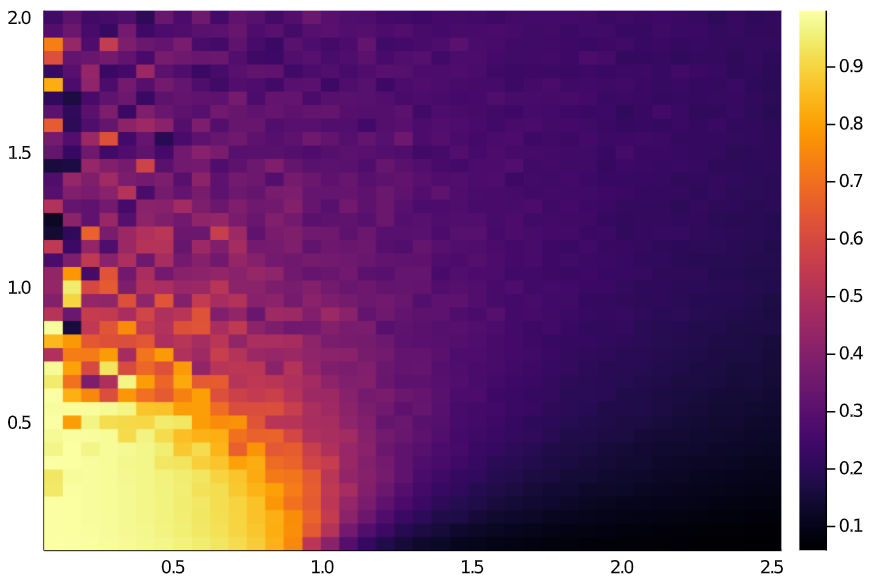
\includegraphics[width=\textwidth]{phase/phase-diagram-transverse-ising-metropolis.PNG}
        \subcaption{}
    \end{subfigure}
    \begin{subfigure}{0.45\textwidth}
        \centering
        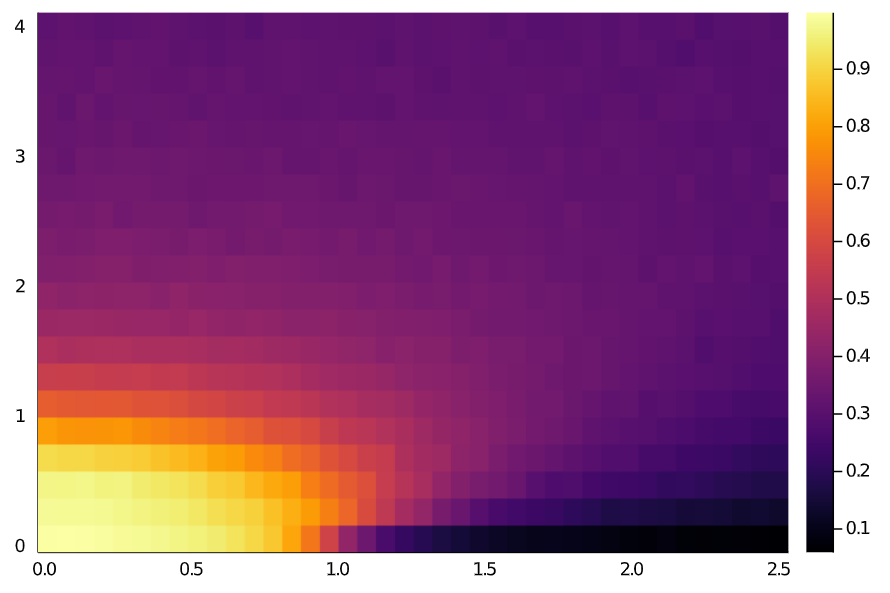
\includegraphics[width=\textwidth]{phase/phase-diagram-transverse-ising-wolff.PNG}
        \subcaption{}
    \end{subfigure}
    \caption{Phase diagrams of 1D transverse field Ising chain obtained with different updating algorithms. The $x$ coordinate is $h$ and the $y$ coordinate is $T$. (a) Metropolis algorithm (b) Wolff cluster algorithm. 
    It can be seen that Metropolis algorithm does not work well when $h$ is small.}
    \label{fig:comparision-metropolis-wolff}
\end{figure}

Since $J_x$ and $J_y$ differ a lot, Metropolis algorithm is incapable for the simulation of the anisotropic Ising model.
Cluster update methods - in this project Wolff cluster updating \cite{Wolff_1989} - must be used.
\prettyref{fig:comparision-metropolis-wolff} shows a comparison between Metropolis algorithm and Wolff algorithm, 
where Metropolis algorithm cannot update the system sufficiently when $h=0$, 
since in that case the 2D \cim corresponding to the 1D transverse field Ising chain degenerates into a classical 1D Ising chain due to the vanishing quantum fluctuation, 
so the coupling strength in the temporal direction approaches to infinite.

\subsection{Monte Carlo simulation of the pure \Ztwo theory's dual transverse field Ising model}

\subsubsection{Benchmark of the algorithms}

\paragraph{Metropolis and Wolff update for \cim}

\begin{figure}
    \centering
    \begin{subfigure}{0.45\textwidth}
        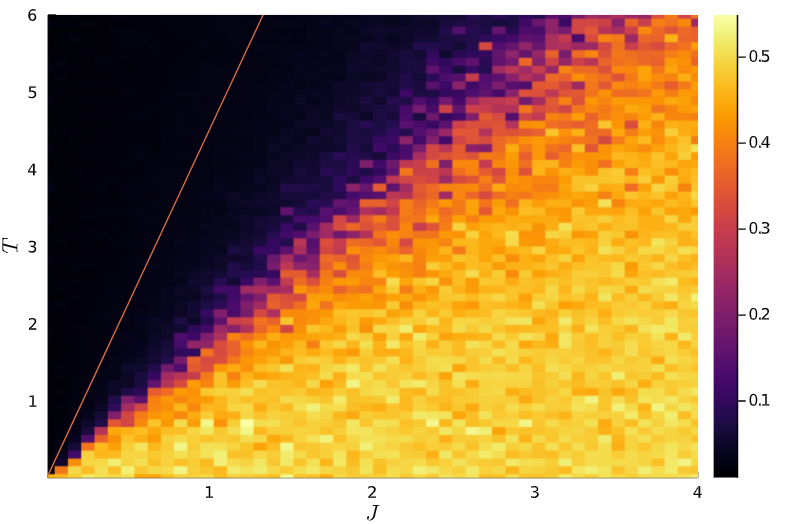
\includegraphics[width=\textwidth]{../3d-ising-prototype/examples/isotropic/magnetization-metropolis-random-init.PNG}
        \subcaption{Metropolis, random initial configuration}
    \end{subfigure}
    \begin{subfigure}{0.45\textwidth}
        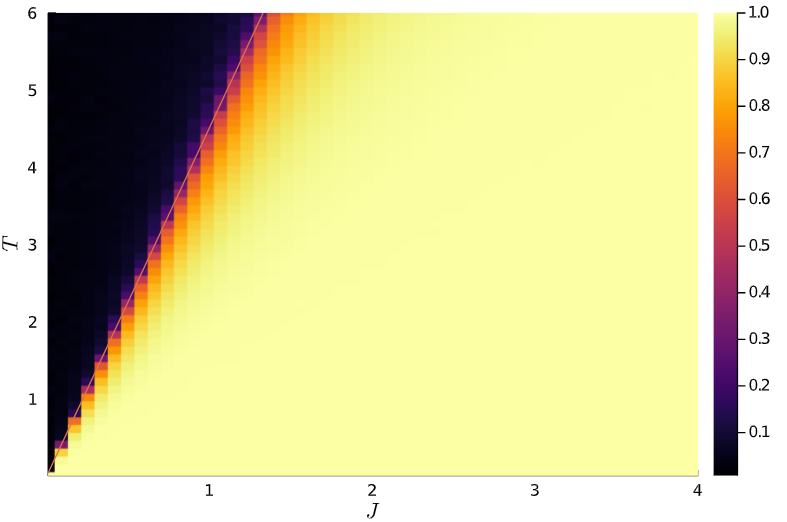
\includegraphics[width=\textwidth]{../3d-ising-prototype/examples/isotropic/magnetization-metropolis-ones-init.PNG}
        \subcaption{Metropolis, initially FM}
    \end{subfigure}
    \begin{subfigure}{0.45\textwidth}
        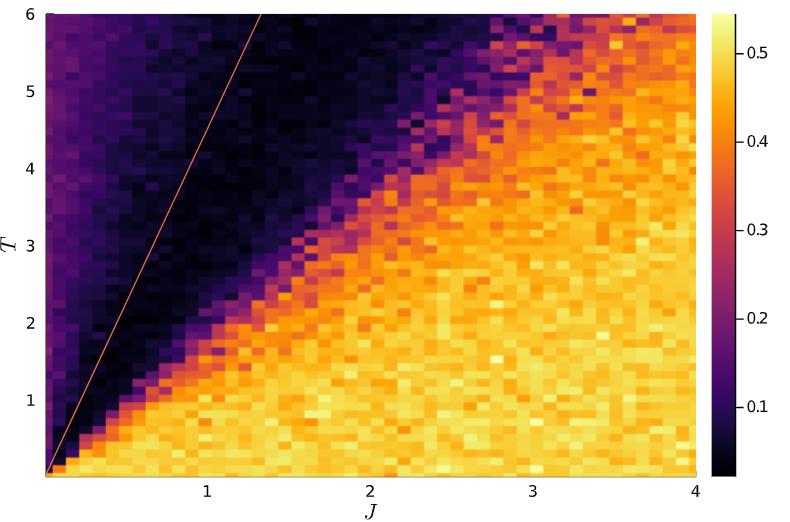
\includegraphics[width=\textwidth]{../3d-ising-prototype/examples/isotropic/magnetization-wolff-random-init.PNG}
        \subcaption{Wolff, random initial configuration}
    \end{subfigure}
    \begin{subfigure}{0.45\textwidth}
        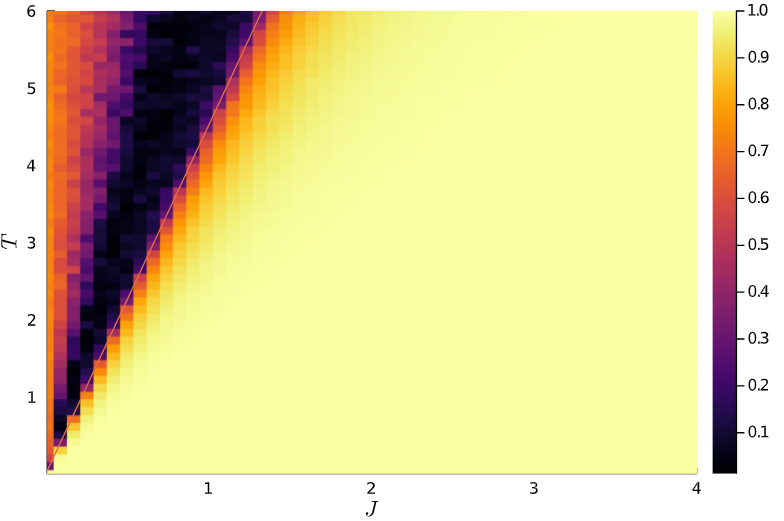
\includegraphics[width=\textwidth]{../3d-ising-prototype/examples/isotropic/magnetization-wolff-ones-init.PNG}
        \subcaption{Wolff, initially FM}
    \end{subfigure}
    \caption{Simulation of 3D \cim using Metropolis update and Wolff update. The data of the straight lines comes from \cite{Talapov_1996}.}
    \label{fig:3d-cim-benchmark}
\end{figure}

\section{Monte Carlo simulation of \eqref{eq:proposed-model}}

\subsection{The \Ztwo gauge theory}

\begin{figure}
    \centering
    

\tikzset{every picture/.style={line width=0.75pt}} %set default line width to 0.75pt        

\begin{tikzpicture}[x=0.75pt,y=0.75pt,yscale=-1,xscale=1]
%uncomment if require: \path (0,300); %set diagram left start at 0, and has height of 300

%Shape: Square [id:dp542262592905693] 
\draw   (180,99) -- (230,99) -- (230,149) -- (180,149) -- cycle ;
%Shape: Square [id:dp09009309223659145] 
\draw   (230,99) -- (280,99) -- (280,149) -- (230,149) -- cycle ;
%Shape: Square [id:dp5226363055605758] 
\draw   (230,149) -- (280,149) -- (280,199) -- (230,199) -- cycle ;
%Shape: Square [id:dp5753693587903983] 
\draw   (280,149) -- (330,149) -- (330,199) -- (280,199) -- cycle ;
%Shape: Square [id:dp2740775722376152] 
\draw   (180,149) -- (230,149) -- (230,199) -- (180,199) -- cycle ;
%Shape: Square [id:dp28430040071015994] 
\draw   (280,99) -- (330,99) -- (330,149) -- (280,149) -- cycle ;
%Straight Lines [id:da3817811530651918] 
\draw [color={rgb, 255:red, 255; green, 50; blue, 0 }  ,draw opacity=1 ]   (180,99) -- (230,99) ;
%Straight Lines [id:da5077651331802149] 
\draw [color={rgb, 255:red, 255; green, 50; blue, 0 }  ,draw opacity=1 ]   (230,99) -- (280,99) ;
%Straight Lines [id:da6234211324926622] 
\draw [color={rgb, 255:red, 255; green, 50; blue, 0 }  ,draw opacity=1 ]   (180,149) -- (230,149) ;
%Straight Lines [id:da9425407569764657] 
\draw [color={rgb, 255:red, 255; green, 50; blue, 0 }  ,draw opacity=1 ]   (230,149) -- (280,149) ;
%Straight Lines [id:da3535261397816505] 
\draw [color={rgb, 255:red, 255; green, 50; blue, 0 }  ,draw opacity=1 ]   (280,99) -- (330,99) ;
%Straight Lines [id:da577016260703958] 
\draw [color={rgb, 255:red, 255; green, 50; blue, 0 }  ,draw opacity=1 ]   (280,149) -- (330,149) ;
%Straight Lines [id:da02814409789415051] 
\draw [color={rgb, 255:red, 255; green, 50; blue, 0 }  ,draw opacity=1 ]   (180,199) -- (230,199) ;
%Straight Lines [id:da4242449962043675] 
\draw [color={rgb, 255:red, 255; green, 50; blue, 0 }  ,draw opacity=1 ]   (230,199) -- (280,199) ;
%Straight Lines [id:da016896896057555955] 
\draw [color={rgb, 255:red, 255; green, 50; blue, 0 }  ,draw opacity=1 ]   (280,199) -- (330,199) ;
%Straight Lines [id:da6633103792674631] 
\draw [color={rgb, 255:red, 0; green, 0; blue, 255 }  ,draw opacity=1 ]   (180,99) -- (180,149) ;
%Straight Lines [id:da8499988857733976] 
\draw [color={rgb, 255:red, 0; green, 0; blue, 255 }  ,draw opacity=1 ]   (180,149) -- (180,199) ;
%Straight Lines [id:da5829594011517594] 
\draw [color={rgb, 255:red, 0; green, 0; blue, 255 }  ,draw opacity=1 ]   (230,99) -- (230,149) ;
%Straight Lines [id:da5372216427388767] 
\draw [color={rgb, 255:red, 0; green, 0; blue, 255 }  ,draw opacity=1 ]   (230,149) -- (230,199) ;
%Straight Lines [id:da4240161703052425] 
\draw [color={rgb, 255:red, 0; green, 0; blue, 255 }  ,draw opacity=1 ]   (280,99) -- (280,149) ;
%Straight Lines [id:da7497455828127941] 
\draw [color={rgb, 255:red, 0; green, 0; blue, 255 }  ,draw opacity=1 ]   (280,149) -- (280,199) ;
%Straight Lines [id:da20504859679327336] 
\draw [color={rgb, 255:red, 0; green, 0; blue, 255 }  ,draw opacity=1 ]   (330,99) -- (330,149) ;
%Straight Lines [id:da40030228249670374] 
\draw [color={rgb, 255:red, 0; green, 0; blue, 255 }  ,draw opacity=1 ]   (330,149) -- (330,199) ;
%Straight Lines [id:da3740769688875947] 
\draw [color={rgb, 255:red, 255; green, 50; blue, 0 }  ,draw opacity=1 ]   (201.64,112.54) -- (207.88,87.4) ;
\draw [shift={(208.36,85.46)}, rotate = 463.92] [fill={rgb, 255:red, 255; green, 50; blue, 0 }  ,fill opacity=1 ][line width=0.08]  [draw opacity=0] (12,-3) -- (0,0) -- (12,3) -- cycle    ;
%Straight Lines [id:da3582938173796022] 
\draw [color={rgb, 255:red, 0; green, 0; blue, 255 }  ,draw opacity=1 ]   (226.64,137.54) -- (232.88,112.4) ;
\draw [shift={(233.36,110.46)}, rotate = 463.92] [fill={rgb, 255:red, 0; green, 0; blue, 255 }  ,fill opacity=1 ][line width=0.08]  [draw opacity=0] (12,-3) -- (0,0) -- (12,3) -- cycle    ;
%Straight Lines [id:da4475629883415315] 
\draw [color={rgb, 255:red, 255; green, 50; blue, 0 }  ,draw opacity=1 ]   (301.64,135.46) -- (307.88,160.6) ;
\draw [shift={(308.36,162.54)}, rotate = 256.08] [fill={rgb, 255:red, 255; green, 50; blue, 0 }  ,fill opacity=1 ][line width=0.08]  [draw opacity=0] (12,-3) -- (0,0) -- (12,3) -- cycle    ;
%Straight Lines [id:da33821278798734755] 
\draw [color={rgb, 255:red, 255; green, 50; blue, 0 }  ,draw opacity=1 ]   (251.64,85.46) -- (257.88,110.6) ;
\draw [shift={(258.36,112.54)}, rotate = 256.08] [fill={rgb, 255:red, 255; green, 50; blue, 0 }  ,fill opacity=1 ][line width=0.08]  [draw opacity=0] (12,-3) -- (0,0) -- (12,3) -- cycle    ;
%Straight Lines [id:da2993789206419337] 
\draw [color={rgb, 255:red, 0; green, 0; blue, 255 }  ,draw opacity=1 ]   (326.64,110.46) -- (332.88,135.6) ;
\draw [shift={(333.36,137.54)}, rotate = 256.08] [fill={rgb, 255:red, 0; green, 0; blue, 255 }  ,fill opacity=1 ][line width=0.08]  [draw opacity=0] (12,-3) -- (0,0) -- (12,3) -- cycle    ;
%Straight Lines [id:da9462772496302772] 
\draw [color={rgb, 255:red, 0; green, 0; blue, 255 }  ,draw opacity=1 ]   (176.64,110.46) -- (182.88,135.6) ;
\draw [shift={(183.36,137.54)}, rotate = 256.08] [fill={rgb, 255:red, 0; green, 0; blue, 255 }  ,fill opacity=1 ][line width=0.08]  [draw opacity=0] (12,-3) -- (0,0) -- (12,3) -- cycle    ;
%Straight Lines [id:da026761975260576776] 
\draw [color={rgb, 255:red, 0; green, 0; blue, 255 }  ,draw opacity=1 ]   (176.64,187.54) -- (182.88,162.4) ;
\draw [shift={(183.36,160.46)}, rotate = 463.92] [fill={rgb, 255:red, 0; green, 0; blue, 255 }  ,fill opacity=1 ][line width=0.08]  [draw opacity=0] (12,-3) -- (0,0) -- (12,3) -- cycle    ;
%Straight Lines [id:da8605119179339802] 
\draw [color={rgb, 255:red, 0; green, 0; blue, 255 }  ,draw opacity=1 ]   (276.64,137.54) -- (282.88,112.4) ;
\draw [shift={(283.36,110.46)}, rotate = 463.92] [fill={rgb, 255:red, 0; green, 0; blue, 255 }  ,fill opacity=1 ][line width=0.08]  [draw opacity=0] (12,-3) -- (0,0) -- (12,3) -- cycle    ;
%Straight Lines [id:da9813428081878903] 
\draw [color={rgb, 255:red, 0; green, 0; blue, 255 }  ,draw opacity=1 ]   (326.64,187.54) -- (332.88,162.4) ;
\draw [shift={(333.36,160.46)}, rotate = 463.92] [fill={rgb, 255:red, 0; green, 0; blue, 255 }  ,fill opacity=1 ][line width=0.08]  [draw opacity=0] (12,-3) -- (0,0) -- (12,3) -- cycle    ;
%Straight Lines [id:da513766484782386] 
\draw [color={rgb, 255:red, 0; green, 0; blue, 255 }  ,draw opacity=1 ]   (276.64,160.46) -- (282.88,185.6) ;
\draw [shift={(283.36,187.54)}, rotate = 256.08] [fill={rgb, 255:red, 0; green, 0; blue, 255 }  ,fill opacity=1 ][line width=0.08]  [draw opacity=0] (12,-3) -- (0,0) -- (12,3) -- cycle    ;
%Straight Lines [id:da16061870084565877] 
\draw [color={rgb, 255:red, 0; green, 0; blue, 255 }  ,draw opacity=1 ]   (226.64,160.46) -- (232.88,185.6) ;
\draw [shift={(233.36,187.54)}, rotate = 256.08] [fill={rgb, 255:red, 0; green, 0; blue, 255 }  ,fill opacity=1 ][line width=0.08]  [draw opacity=0] (12,-3) -- (0,0) -- (12,3) -- cycle    ;
%Straight Lines [id:da04950197329891548] 
\draw [color={rgb, 255:red, 255; green, 50; blue, 0 }  ,draw opacity=1 ]   (251.64,162.54) -- (257.88,137.4) ;
\draw [shift={(258.36,135.46)}, rotate = 463.92] [fill={rgb, 255:red, 255; green, 50; blue, 0 }  ,fill opacity=1 ][line width=0.08]  [draw opacity=0] (12,-3) -- (0,0) -- (12,3) -- cycle    ;
%Straight Lines [id:da06768946495338946] 
\draw [color={rgb, 255:red, 255; green, 50; blue, 0 }  ,draw opacity=1 ]   (301.64,85.46) -- (307.88,110.6) ;
\draw [shift={(308.36,112.54)}, rotate = 256.08] [fill={rgb, 255:red, 255; green, 50; blue, 0 }  ,fill opacity=1 ][line width=0.08]  [draw opacity=0] (12,-3) -- (0,0) -- (12,3) -- cycle    ;
%Straight Lines [id:da19487888642782658] 
\draw [color={rgb, 255:red, 255; green, 50; blue, 0 }  ,draw opacity=1 ]   (201.64,135.46) -- (207.88,160.6) ;
\draw [shift={(208.36,162.54)}, rotate = 256.08] [fill={rgb, 255:red, 255; green, 50; blue, 0 }  ,fill opacity=1 ][line width=0.08]  [draw opacity=0] (12,-3) -- (0,0) -- (12,3) -- cycle    ;
%Straight Lines [id:da9921787419722914] 
\draw    (157.33,237.67) -- (205.33,237.67) ;
\draw [shift={(207.33,237.67)}, rotate = 180] [fill={rgb, 255:red, 0; green, 0; blue, 0 }  ][line width=0.08]  [draw opacity=0] (12,-3) -- (0,0) -- (12,3) -- cycle    ;
%Straight Lines [id:da18519953870442474] 
\draw    (157.33,237.67) -- (157.33,189.67) ;
\draw [shift={(157.33,187.67)}, rotate = 450] [fill={rgb, 255:red, 0; green, 0; blue, 0 }  ][line width=0.08]  [draw opacity=0] (12,-3) -- (0,0) -- (12,3) -- cycle    ;

% Text Node
\draw (58.67,104.57) node [anchor=north west][inner sep=0.75pt]    {$ \begin{array}{l}
\textcolor[rgb]{1,0.2,0}{\sigma }\textcolor[rgb]{1,0.2,0}{_{\boldsymbol{i} A}}\textcolor[rgb]{1,0.2,0}{=+1}\\
\textcolor[rgb]{0,0,1}{\sigma }\textcolor[rgb]{0,0,1}{_{\boldsymbol{i} B}}\textcolor[rgb]{0,0,1}{=-1}\\
\textcolor[rgb]{1,0.2,0}{\sigma }\textcolor[rgb]{1,0.2,0}{_{\boldsymbol{j} A}}\textcolor[rgb]{1,0.2,0}{=-1}\\
\textcolor[rgb]{0,0,1}{\sigma }\textcolor[rgb]{0,0,1}{_{\boldsymbol{j} B}}\textcolor[rgb]{0,0,1}{=+1}
\end{array}$};
% Text Node
\draw (178,95.6) node [anchor=south east] [inner sep=0.75pt]    {$\boldsymbol{i}$};
% Text Node
\draw (230,92.6) node [anchor=south] [inner sep=0.75pt]    {$\boldsymbol{j}$};
% Text Node
\draw (209.33,237.67) node [anchor=west] [inner sep=0.75pt]    {$x$};
% Text Node
\draw (157.45,184.27) node [anchor=south] [inner sep=0.75pt]  [rotate=-2]  {$y$};


\end{tikzpicture}

    \caption{Dividing a gauge field configuration into two sublattices}
    \label{fig:z2-dividing}
\end{figure}

\Ztwo gauge degrees of freedom are defined on bonds. 
Suppose there are $N$ sites. Since there are 4 bonds connecting to one site and a bond is shared by two sites,
there are $4 N / 2 = 2 N$ bonds.
Therefore, the \Ztwo gauge degrees of freedom can be divided into two sublattices, each of which has $N$ degrees of freedom, shown in \prettyref{fig:z2-dividing}.
Actually in order to be consistent with Julia's array indexing convention, we choose \prettyref{fig:z2-dividing-real} as our convention to label the \Ztwo gauge degrees of freedom.
Note that the definition of A sublattice and B sublattice in \prettyref{fig:z2-dividing} is exactly opposite to the definition in \prettyref{fig:z2-dividing-real}.

\begin{figure}
    \centering
    

\tikzset{every picture/.style={line width=0.75pt}} %set default line width to 0.75pt        

\begin{tikzpicture}[x=0.75pt,y=0.75pt,yscale=-1,xscale=1]
%uncomment if require: \path (0,300); %set diagram left start at 0, and has height of 300

%Shape: Square [id:dp94343580808897] 
\draw   (148,79) -- (198,79) -- (198,129) -- (148,129) -- cycle ;
%Shape: Square [id:dp904320118364085] 
\draw   (198,79) -- (248,79) -- (248,129) -- (198,129) -- cycle ;
%Shape: Square [id:dp23810340973583366] 
\draw   (198,129) -- (248,129) -- (248,179) -- (198,179) -- cycle ;
%Shape: Square [id:dp7442875383350216] 
\draw   (248,129) -- (298,129) -- (298,179) -- (248,179) -- cycle ;
%Shape: Square [id:dp6778551563517383] 
\draw   (148,129) -- (198,129) -- (198,179) -- (148,179) -- cycle ;
%Shape: Square [id:dp6416389603622314] 
\draw   (248,79) -- (298,79) -- (298,129) -- (248,129) -- cycle ;
%Straight Lines [id:da33987514617833803] 
\draw [color={rgb, 255:red, 255; green, 50; blue, 0 }  ,draw opacity=1 ]   (148,79) -- (198,79) ;
%Straight Lines [id:da4754714420859858] 
\draw [color={rgb, 255:red, 255; green, 50; blue, 0 }  ,draw opacity=1 ]   (198,79) -- (248,79) ;
%Straight Lines [id:da8288457368423472] 
\draw [color={rgb, 255:red, 255; green, 50; blue, 0 }  ,draw opacity=1 ]   (148,129) -- (198,129) ;
%Straight Lines [id:da8766911392918253] 
\draw [color={rgb, 255:red, 255; green, 50; blue, 0 }  ,draw opacity=1 ]   (198,129) -- (248,129) ;
%Straight Lines [id:da7976747716122397] 
\draw [color={rgb, 255:red, 255; green, 50; blue, 0 }  ,draw opacity=1 ]   (248,79) -- (298,79) ;
%Straight Lines [id:da6261387523555471] 
\draw [color={rgb, 255:red, 255; green, 50; blue, 0 }  ,draw opacity=1 ]   (248,129) -- (298,129) ;
%Straight Lines [id:da5123484057107612] 
\draw [color={rgb, 255:red, 255; green, 50; blue, 0 }  ,draw opacity=1 ]   (148,179) -- (198,179) ;
%Straight Lines [id:da8943057989577798] 
\draw [color={rgb, 255:red, 255; green, 50; blue, 0 }  ,draw opacity=1 ]   (198,179) -- (248,179) ;
%Straight Lines [id:da32774689246333755] 
\draw [color={rgb, 255:red, 255; green, 50; blue, 0 }  ,draw opacity=1 ]   (248,179) -- (298,179) ;
%Straight Lines [id:da5238661994412872] 
\draw [color={rgb, 255:red, 0; green, 0; blue, 255 }  ,draw opacity=1 ]   (148,79) -- (148,129) ;
%Straight Lines [id:da04206179047427416] 
\draw [color={rgb, 255:red, 0; green, 0; blue, 255 }  ,draw opacity=1 ]   (148,129) -- (148,179) ;
%Straight Lines [id:da25559494537897476] 
\draw [color={rgb, 255:red, 0; green, 0; blue, 255 }  ,draw opacity=1 ]   (198,79) -- (198,129) ;
%Straight Lines [id:da6710293145780648] 
\draw [color={rgb, 255:red, 0; green, 0; blue, 255 }  ,draw opacity=1 ]   (198,129) -- (198,179) ;
%Straight Lines [id:da049098956500436275] 
\draw [color={rgb, 255:red, 0; green, 0; blue, 255 }  ,draw opacity=1 ]   (248,79) -- (248,129) ;
%Straight Lines [id:da5445404258762208] 
\draw [color={rgb, 255:red, 0; green, 0; blue, 255 }  ,draw opacity=1 ]   (248,129) -- (248,179) ;
%Straight Lines [id:da5961190608463656] 
\draw [color={rgb, 255:red, 0; green, 0; blue, 255 }  ,draw opacity=1 ]   (298,79) -- (298,129) ;
%Straight Lines [id:da999070039134085] 
\draw [color={rgb, 255:red, 0; green, 0; blue, 255 }  ,draw opacity=1 ]   (298,129) -- (298,179) ;
%Straight Lines [id:da1555476489184353] 
\draw [color={rgb, 255:red, 255; green, 50; blue, 0 }  ,draw opacity=1 ]   (169.64,92.54) -- (175.88,67.4) ;
\draw [shift={(176.36,65.46)}, rotate = 463.92] [fill={rgb, 255:red, 255; green, 50; blue, 0 }  ,fill opacity=1 ][line width=0.08]  [draw opacity=0] (12,-3) -- (0,0) -- (12,3) -- cycle    ;
%Straight Lines [id:da5588828730404596] 
\draw [color={rgb, 255:red, 0; green, 0; blue, 255 }  ,draw opacity=1 ]   (194.64,117.54) -- (200.88,92.4) ;
\draw [shift={(201.36,90.46)}, rotate = 463.92] [fill={rgb, 255:red, 0; green, 0; blue, 255 }  ,fill opacity=1 ][line width=0.08]  [draw opacity=0] (12,-3) -- (0,0) -- (12,3) -- cycle    ;
%Straight Lines [id:da6025879618253642] 
\draw [color={rgb, 255:red, 255; green, 50; blue, 0 }  ,draw opacity=1 ]   (269.64,115.46) -- (275.88,140.6) ;
\draw [shift={(276.36,142.54)}, rotate = 256.08] [fill={rgb, 255:red, 255; green, 50; blue, 0 }  ,fill opacity=1 ][line width=0.08]  [draw opacity=0] (12,-3) -- (0,0) -- (12,3) -- cycle    ;
%Straight Lines [id:da12771191721633213] 
\draw [color={rgb, 255:red, 255; green, 50; blue, 0 }  ,draw opacity=1 ]   (219.64,65.46) -- (225.88,90.6) ;
\draw [shift={(226.36,92.54)}, rotate = 256.08] [fill={rgb, 255:red, 255; green, 50; blue, 0 }  ,fill opacity=1 ][line width=0.08]  [draw opacity=0] (12,-3) -- (0,0) -- (12,3) -- cycle    ;
%Straight Lines [id:da25131845224806093] 
\draw [color={rgb, 255:red, 0; green, 0; blue, 255 }  ,draw opacity=1 ]   (294.64,90.46) -- (300.88,115.6) ;
\draw [shift={(301.36,117.54)}, rotate = 256.08] [fill={rgb, 255:red, 0; green, 0; blue, 255 }  ,fill opacity=1 ][line width=0.08]  [draw opacity=0] (12,-3) -- (0,0) -- (12,3) -- cycle    ;
%Straight Lines [id:da11876088311135646] 
\draw [color={rgb, 255:red, 0; green, 0; blue, 255 }  ,draw opacity=1 ]   (144.64,90.46) -- (150.88,115.6) ;
\draw [shift={(151.36,117.54)}, rotate = 256.08] [fill={rgb, 255:red, 0; green, 0; blue, 255 }  ,fill opacity=1 ][line width=0.08]  [draw opacity=0] (12,-3) -- (0,0) -- (12,3) -- cycle    ;
%Straight Lines [id:da6890864290010354] 
\draw [color={rgb, 255:red, 0; green, 0; blue, 255 }  ,draw opacity=1 ]   (144.64,167.54) -- (150.88,142.4) ;
\draw [shift={(151.36,140.46)}, rotate = 463.92] [fill={rgb, 255:red, 0; green, 0; blue, 255 }  ,fill opacity=1 ][line width=0.08]  [draw opacity=0] (12,-3) -- (0,0) -- (12,3) -- cycle    ;
%Straight Lines [id:da05289574132290853] 
\draw [color={rgb, 255:red, 0; green, 0; blue, 255 }  ,draw opacity=1 ]   (244.64,117.54) -- (250.88,92.4) ;
\draw [shift={(251.36,90.46)}, rotate = 463.92] [fill={rgb, 255:red, 0; green, 0; blue, 255 }  ,fill opacity=1 ][line width=0.08]  [draw opacity=0] (12,-3) -- (0,0) -- (12,3) -- cycle    ;
%Straight Lines [id:da21476740161555674] 
\draw [color={rgb, 255:red, 0; green, 0; blue, 255 }  ,draw opacity=1 ]   (294.64,167.54) -- (300.88,142.4) ;
\draw [shift={(301.36,140.46)}, rotate = 463.92] [fill={rgb, 255:red, 0; green, 0; blue, 255 }  ,fill opacity=1 ][line width=0.08]  [draw opacity=0] (12,-3) -- (0,0) -- (12,3) -- cycle    ;
%Straight Lines [id:da7136915390220577] 
\draw [color={rgb, 255:red, 0; green, 0; blue, 255 }  ,draw opacity=1 ]   (244.64,140.46) -- (250.88,165.6) ;
\draw [shift={(251.36,167.54)}, rotate = 256.08] [fill={rgb, 255:red, 0; green, 0; blue, 255 }  ,fill opacity=1 ][line width=0.08]  [draw opacity=0] (12,-3) -- (0,0) -- (12,3) -- cycle    ;
%Straight Lines [id:da48675572724238214] 
\draw [color={rgb, 255:red, 0; green, 0; blue, 255 }  ,draw opacity=1 ]   (194.64,140.46) -- (200.88,165.6) ;
\draw [shift={(201.36,167.54)}, rotate = 256.08] [fill={rgb, 255:red, 0; green, 0; blue, 255 }  ,fill opacity=1 ][line width=0.08]  [draw opacity=0] (12,-3) -- (0,0) -- (12,3) -- cycle    ;
%Straight Lines [id:da7549121433002168] 
\draw [color={rgb, 255:red, 255; green, 50; blue, 0 }  ,draw opacity=1 ]   (219.64,142.54) -- (225.88,117.4) ;
\draw [shift={(226.36,115.46)}, rotate = 463.92] [fill={rgb, 255:red, 255; green, 50; blue, 0 }  ,fill opacity=1 ][line width=0.08]  [draw opacity=0] (12,-3) -- (0,0) -- (12,3) -- cycle    ;
%Straight Lines [id:da8715022833218335] 
\draw    (112,36) -- (112,149.31) ;
\draw [shift={(112,151.31)}, rotate = 270] [fill={rgb, 255:red, 0; green, 0; blue, 0 }  ][line width=0.08]  [draw opacity=0] (12,-3) -- (0,0) -- (12,3) -- cycle    ;
%Straight Lines [id:da445086367084234] 
\draw    (112,36) -- (264.81,36) ;
\draw [shift={(266.81,36)}, rotate = 180] [fill={rgb, 255:red, 0; green, 0; blue, 0 }  ][line width=0.08]  [draw opacity=0] (12,-3) -- (0,0) -- (12,3) -- cycle    ;

%Straight Lines [id:da2184148875244607] 
\draw [color={rgb, 255:red, 255; green, 50; blue, 0 }  ,draw opacity=1 ]   (269.64,65.46) -- (275.88,90.6) ;
\draw [shift={(276.36,92.54)}, rotate = 256.08] [fill={rgb, 255:red, 255; green, 50; blue, 0 }  ,fill opacity=1 ][line width=0.08]  [draw opacity=0] (12,-3) -- (0,0) -- (12,3) -- cycle    ;
%Straight Lines [id:da11157936961811532] 
\draw [color={rgb, 255:red, 255; green, 50; blue, 0 }  ,draw opacity=1 ]   (169.64,115.46) -- (175.88,140.6) ;
\draw [shift={(176.36,142.54)}, rotate = 256.08] [fill={rgb, 255:red, 255; green, 50; blue, 0 }  ,fill opacity=1 ][line width=0.08]  [draw opacity=0] (12,-3) -- (0,0) -- (12,3) -- cycle    ;

% Text Node
\draw (10,75.9) node [anchor=north west][inner sep=0.75pt]    {$ \begin{array}{l}
\textcolor[rgb]{1,0.2,0}{\sigma }\textcolor[rgb]{1,0.2,0}{_{\boldsymbol{i} A}}\textcolor[rgb]{1,0.2,0}{=+1}\\
\textcolor[rgb]{0,0,1}{\sigma }\textcolor[rgb]{0,0,1}{_{\boldsymbol{i} B}}\textcolor[rgb]{0,0,1}{=-1}\\
\textcolor[rgb]{1,0.2,0}{\sigma }\textcolor[rgb]{1,0.2,0}{_{\boldsymbol{j} A}}\textcolor[rgb]{1,0.2,0}{=-1}\\
\textcolor[rgb]{0,0,1}{\sigma }\textcolor[rgb]{0,0,1}{_{\boldsymbol{j} B}}\textcolor[rgb]{0,0,1}{=+1}
\end{array}$};
% Text Node
\draw (146,75.6) node [anchor=south east] [inner sep=0.75pt]    {$\boldsymbol{i}$};
% Text Node
\draw (198,72.6) node [anchor=south] [inner sep=0.75pt]    {$\boldsymbol{j}$};
% Text Node
\draw (112,154.71) node [anchor=north] [inner sep=0.75pt]    {$x$};
% Text Node
\draw (268.81,36) node [anchor=west] [inner sep=0.75pt]    {$y$};


\end{tikzpicture}

    \caption{Another way to divide a gauge field configuration into two sublattices, in agreement with Julia's index convention, where \texttt{i} in \texttt{...[i, j]} means $x$ and \texttt{j} means $y$.}
    \label{fig:z2-dividing-real}
\end{figure}

\subsection{Fermions}

The way to update fermions can be found in the appendix of \cite{Chen_2021}.

\bibliographystyle{plain}
\bibliography{note} 

\end{document}